\begin{flushright} {\tiny {\color{gray} cvi.tex}} \end{flushright}
%~~~~~~~~~~~~~~~~~~~~~~~~~~~~~~~~~~~~~~~~~~~~~~~~~~~~~~~~~~~~~~~~~~~~~~~~~~~~~~~~~~~~~~~~~~~~~~~~~~


To my knowledge the conservative velocity interpolation (CVI) was introduced to 
the computational geodynamics community in Wang \etal (2015) \cite{waav15}. 
As mentioned in the paper 
``An improved velocity interpolation scheme that conserves the divergence of the flow field has 
been developed by Jenny \etal (2001) \cite{jepm01} and the simplified scheme for incompressible 
flow (i.e., divergence free) has been demonstrated that it largely eliminates the spurious 
distribution of particles for 2D incompressible flow problem (see Meyer and Jenny (2004) \cite{meje04}).''

%-------------------------------------------------------------
\subsubsection{A few remarks about Wang \etal (2015)}

The article by Wang \etal (2015) comes with supplementary material with more details on the 
derivation of the corrective velocities but that material is a Word
document printed to pdf with an annoying layout of equations, different font sizes,
lack of alignment, etc ... 
Also, Fig.~1 of the paper is reproduced here:
\begin{center}
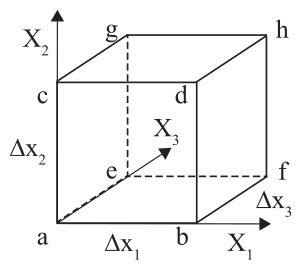
\includegraphics[width=4cm]{images/cvi/wang15}
\end{center}
Why the authors chose to label nodes a,b,...h and not 1,2,...8 shall forever remain 
a mystery, but it is not as problematic as the labelling of the axes:
indeed, if $X_1$ is the $x$-axis then $X_3$ should be the $y$-axis 
and $X_2$ the $z$-axis. That is quite illogical. Or is it a mistake in 
the drawing only? In any case this sheds some confusion on the equations 
presented in the paper so I have decided to carry out all the CVI derivations 
in this chapter.

Their paper does not seem to consider cases where the element is not a 
cuboid (so what about CitcomS, or ALE formulations?), nor does it address higher order elements. 
Finally many details of the setups in the paper are just not there and I had to 
email the author(s) multiple time regarding:

\begin{itemize}
\item the setup of the couette flow in section 3.1 is 
incomplete: for instance, size of the box ? velocity value ? exact 
formula for the vel field (couette flow, I know, but how thick are the 
layers before rotation)? etc ...\\
Wang answered me: ``The box is a unit box (nondimentional 1*1). I attached the function for 
the analytical solution for the exact formula for the velocity field that you asked. I didn't 
find the models file yet, so I can't tell you what it is the value of the velocity. 
But I think it can be: 1m*1m box with 1m/s on the surface (V0).
In Citcom, the timestep is chosen to let any material in one cell not to move more than half
of the cell length (CFL=0.5). Then we have this parameter "finetunedt" ($<1$) to multiply it. I remember
I usually use 0.9 or 0.7.  So the CFL=0.45 or 0.35. 
Concerning the Couette flow we used a viscosity of 1e3, 
which make very sharp velocity contrast across the diagonal line.''
\begin{small}
\begin{verbatim}
for (i=1;i<=E->lmesh.nno;i++)
{     
x =  E->X[1][i]; 
z =  E->X[2][i];
eta1=E->control.testvelval[1];
eta2=E->control.testvelval[2];
alpha=E->control.testvelval[3]*PI/180;  /*coordinate rotation angle */
V0=E->control.testvelval[4];
h=sqrt(2.0)*sin(alpha+PI/4); /*WHL: h (with analytical solution) is a function of the rotation angle */
V1=(x*sin(alpha)+z*cos(alpha))*2*V0*eta2/(eta1+eta2)/h;
V2=(x*sin(alpha)+z*cos(alpha))*2*V0*eta1/(eta1+eta2)/h+(eta2-eta1)*V0/(eta1+eta2);
if (x*sin(alpha)+z*cos(alpha)<0.5*h)          
{
E->V[1][i]=V1*cos(alpha);
E->V[2][i]=-V1*sin(alpha);
}
else
{
E->V[1][i]=V2*cos(alpha);
E->V[2][i]=-V2*sin(alpha);
}
if (E->mesh.nsd == 3)
E->V[3][i]=0.;
}
\end{verbatim}
\end{small}

\item which advection scheme was used and 
I am worried that at no point in the publication the timestep size is 
either mentioned nor its importance discussed.\\
Wang answered: ``About the timestep, my experience is that using smaller timestep 
would't solve this kind of problem. Otherwise we probably
would not need to use this new velocity interpolation.  I could not remember that I tested 
the effects of timestep for this model. So it would be nice to know the result if you test it.  
The advection scheme is the 2nd Runge Kutta. ''

\item Agrusta wrote: "here the input values for the couette flow: 
testvelval=100000,1,45,0.01    \# eta1,eta2,angle,velocity. mesh = 33x33. 
initial tracers 100X100, random distribution"

\end{itemize}

Looking at their Fig.~2a,b we see black arrow tips in the blue region where 
velocity should be zero. Velocity is indeed zero and the authors confirmed that 
the arrow tips are an artefact of their visualisation software (!).

\Literature: 
McNally (2011) \cite{mcna11} proposed
a divergence-free interpolation of vector fields from point values in the context 
of magnetohydrodynamics.
Pusok \etal (2016) \cite{pukp16} has applied the CVI to staggered grid FDM.

 
%-------------------------------------------------------------
\subsubsection{In 2D with $Q_1$ basis functions - Naive approach}

Let us start directly in reduced coordinates $(r,s)\in [-1:1]^2$ (i.e. the reference element).
The velocity components inside of the element are given by:
\begin{eqnarray}
u^h(r,s)&=&\sum_i \bN_i(r,s) u_i \nn\\
v^h(r,s)&=&\sum_i \bN_i(r,s) v_i \nn
\end{eqnarray}
where $\bN_i$ are the four $Q_1$ basis functions defined as follows:
\begin{eqnarray}
\bN_1(r,s)&=& \frac{1}{4}(1-r)(1-s)  \nonumber\\ 
\bN_2(r,s)&=& \frac{1}{4}(1+r)(1-s)  \nonumber\\ 
\bN_3(r,s)&=& \frac{1}{4}(1+r)(1+s)  \nonumber\\ 
\bN_4(r,s)&=& \frac{1}{4}(1-r)(1+s)  \nonumber
\end{eqnarray}
The incompressibility constraint in the $(r,s)-$coordinate system reads
\[
(\vec\nabla\cdot\vec\upnu)^h=
\frac{\partial u^h}{\partial r}+
\frac{\partial v^h}{\partial s}
=
\sum_i \left(  
\frac{\partial \bN_i}{\partial r} u_i+
\frac{\partial \bN_i}{\partial s} v_i
\right)
=0.
\]
However, it is trivial to verify that the incompressibility 
condition is not and \textit{can not} be verified for all values of  
$r,s \in [-1,1]^2$.
It would then make sense to think of a corrective term to the interpolation
which would add just enough degrees of freedoms so as to insure an exact\footnote{more
on this later} incompressibility in the element. 
Let us then write:
\begin{eqnarray}
u^h(r,s)&=&\sum_i \bN_i(r,s) u_i + (a s + b)(1-r)(1+r) \nn\\
v^h(r,s)&=&\sum_i \bN_i(r,s) v_i + (c r + d)(1-s)(1+s) \nn
\end{eqnarray}
Note that in this way the correction is zero on the $x=-1$ and $x=+1$ sides 
of the element for $u$, and likewise for $v$ on the top and bottom sides (in 
other words the velocity remains continuous from one element to another).
In this case,
\begin{eqnarray}
\frac{\partial u^h}{\partial r}&=&\sum_i \frac{\partial \bN_i}{\partial r} u_i + (a s + b) (-2r) \nn\\
\frac{\partial v^h}{\partial s}&=&\sum_i \frac{\partial \bN_i}{\partial s} v_i + (c r + d)(-2s) \nn
\end{eqnarray}
We have introduced 4 coefficients  $(a,b,c,d)$ which remain to be determined. 
We start with:
\begin{eqnarray}
\sum_i \frac{\partial N_i}{\partial r} u_i 
&=& -\frac{1}{4} (1-s) u_1 + \frac{1}{4} (1-s) u_2 +\frac{1}{4} (1+s) u_3 -\frac{1}{4} (1+s) u_4 \nn\\
&=& (1-s) \frac{u_2-u_1}{4} + (1+s) \frac{u_3-u_4}{4} \nn\\
&=& (1-s) u_{21} + (1+s) u_{34} \nn\\
\sum_i \frac{\partial N_i}{\partial s} v_i 
&=& -\frac{1}{4} (1-r) v_1 - \frac{1}{4} (1+r) v_2 +\frac{1}{4} (1+r) v_3 +\frac{1}{4} (1-r) v_4 \nn\\
&=& (1-r) \frac{v_4-v_1}{4} + (1+r)\frac{v_3-v_2}{4} \nn\\
&=& (1-r) v_{41} + (1+r) v_{32} \nn
\end{eqnarray}
where $u_{ij}=(u_i-u_j)/4$ and $v_{ij}=(v_i-v_j)/4$, so that in the end
\begin{eqnarray}
\frac{\partial u^h}{\partial r} &=& (1-s) u_{21} + (1+s) u_{34} + (a s + b)(-2r) \\
\frac{\partial v^h}{\partial s} &=& (1-r) v_{41} + (1+r) v_{32} + (c r + d)(-2s)
\end{eqnarray}
The incompressibility condition is now:
\[
(\vec\nabla\cdot\vec\upnu)^h =
(1-s) u_{21} + (1+s) u_{34} 
+ (a s + b) (-2r) +
(1-r) v_{41} + (1+r) v_{32}
+ (c r + d)(-2s)
=0
\]
This can be rewritten as
\[
(\vec\nabla\cdot\vec\upnu)^h =
C_0  + C_1 r + C_2 s + C_3 rs = 0
\]
where the four $C_i$ coefficients are functions of the velocities and the other coefficients.
In order for this expression to be exactly zero {\it everywhere}, each $C$ coefficient has
to be independently zero.

\begin{eqnarray}
C_0   &(.)  &  u_{21} + u_{34} + v_{41} + v_{32} =0\nn\\ 
C_1   &(r)  &  -v_{41} + v_{32} -2b =0\nn\\ 
C_2   &(s)  &  -u_{21} + u_{34} -2d =0 \nn\\ 
C_3   &(rs) &  -2a -2c =0\nn 
\end{eqnarray}

The first line is simply the incompressibility condition
expressed in the center of the element (i.e. $r=s=0$),
so we set it aside for now (I will come back to it later!)
and focus on the remaining three.

At this stage it is important to note that in the absence of corrective terms (i.e. $a=b=c=d=0$)
then only $C_3=0$ and the divergence inside the element is a linear field.

We obtain
\[
c=-a
\qquad
b=\frac{1}{2}(-v_{41} + v_{32})
\qquad
d=\frac{1}{2} (-u_{21} + u_{34})
\]
Since $a$ and $c$ are not otherwise constrained, we can set them to zero, and we then have:
\[
b=\frac{1}{2}(v_{14} + v_{32})
\quad\quad
d=\frac{1}{2} (u_{12} + u_{34})
\]
and finally
\begin{eqnarray}
u^h(r,s)
&=&\sum_i \bN_i(r,s) u_i + b(1-r)(1+r) 
=\sum_i \bN_i(r,s) u_i + \frac{1}{2}(v_{14} + v_{32})(1-r)(1+r) \nn\\
v^h(r,s)
&=&\sum_i \bN_i(r,s) v_i + d(1-s)(1+s) 
=\sum_i \bN_i(r,s) v_i + \frac{1}{2} (u_{12} + u_{34})(1-s)(1+s) \nn
\end{eqnarray}

By using these corrected interpolations for both components 
of the velocity then one ensures that a point-wise divergence free
velocity field anywhere in the element.
However, these derivations were carried out in the reference element. 
In fact they would work also for rectangular elements with minimal 
changes, but not for generic quadrilaterals.

To be clear, let us now compute the velocity divergence of the corrected 
velocity field above:
\begin{eqnarray}
(\vec\nabla\cdot\vec\upnu)^h 
&=&
\frac{\partial u^h}{\partial r}+
\frac{\partial v^h}{\partial s}
\nn\\
&=& (1-s) u_{21} + (1+s) u_{34} +  \frac{1}{2}(v_{14} + v_{32})(-2r)
+ (1-r) v_{41} + (1+r) v_{32}  + \frac{1}{2} (u_{12} + u_{34})(-2s) \nn\\
&=& u_{21} + u_{34} + v_{41} + v_{32}
-s u_{21} + s u_{34} -r v_{14} -r v_{32} 
-r v_{41} + r v_{32} -s u_{12} -s u_{34} \nn\\
&=& u_{21} + u_{34} + v_{41} + v_{32} 
\end{eqnarray}
A point must then be made crystal clear: the divergence is
{\it not} zero. The quantity above is constant inside the element 
(it does not depend on $r$ nor $s$). 
All what the CVI algorithm does is to remove the spatial dependence
of the velocity divergence inside the element.

%-------------------------------------------------------------------
\subsubsection{In 2D with $Q_1$ basis functions - better approach}

We now consider a generic quadrilateral in the $x,y$-coordinate space and its equivalent in the 
reference space $r,s$. One can easily show that the gradient of a field $f$ verifies 
\[
\left(
\begin{array}{c}
\frac{\partial f}{\partial x} \\ \\
\frac{\partial f}{\partial y} 
\end{array}
\right)
=
\tilde{\bm J} \cdot
\left(
\begin{array}{c}
\frac{\partial f}{\partial r} \\ \\
\frac{\partial f}{\partial s} 
\end{array}
\right)
\]
where $\tilde{\bm J}$ in the inverse of the Jacobian matrix.
We then postulate again
\begin{eqnarray}
u^h(r,s)&=&\sum_i \bN_i(r,s) u_i + (a s + b)(1-r)(1+r) \nn\\
v^h(r,s)&=&\sum_i \bN_i(r,s) v_i + (c r + d)(1-s)(1+s) \nn
\end{eqnarray}
In this case,
\begin{eqnarray}
\frac{\partial u^h}{\partial r}&=&\sum_i \frac{\partial \bN_i}{\partial r} u_i + (a s + b) (-2r)   \nn\\
\frac{\partial u^h}{\partial s}&=&\sum_i \frac{\partial \bN_i}{\partial s} u_i + a (1-r^2) \nn\\
\frac{\partial v^h}{\partial r}&=&\sum_i \frac{\partial \bN_i}{\partial s} v_i + c (1-s^2) \nn\\
\frac{\partial v^h}{\partial s}&=&\sum_i \frac{\partial \bN_i}{\partial s} v_i + (c r + d)(-2s) \nn
\end{eqnarray}
We have introduced 4 coefficients  $(a,b,c,d)$ which remain to be determined.
In order to compute the velocity divergence inside the element we will need 
\begin{eqnarray}
\frac{\partial u}{\partial x} 
&=& \tilde{J}_{xx} \frac{\partial u}{\partial r} +  \tilde{J}_{xy} \frac{\partial u}{\partial s}  \nn\\
&=& \tilde{J}_{xx} \left( \sum_i \frac{\partial \bN_i}{\partial r} u_i + (a s + b) (-2r)  \right) 
 +  \tilde{J}_{xy} \left( \sum_i \frac{\partial \bN_i}{\partial s} u_i + a (1-r^2) \right)  \nn\\
&=& \tilde{J}_{xx} \left(  -(1-s) u_{12} + (1+s) u_{34} + (a s + b) (-2r)  \right) \nn\\ 
&+&  \tilde{J}_{xy} \left(  -(1-r) u_{14} - (1+r) u_{23} + a (1-r^2) \right)
\nn\\
\frac{\partial v}{\partial y} 
&=& \tilde{J}_{yx} \left(  -(1-s) v_{12} + (1+s) v_{34} + c (1-s^2)   \right)  \nn\\
&+&  \tilde{J}_{yy} \left(  -(1-r) v_{14} - (1+r) v_{23} + (cr+d) (-2s) \right) \nn
\end{eqnarray}
where $u_{ij}=(u_i-u_j)/4$ and $v_{ij}=(v_i-v_j)/4$.
The velocity divergence can be written as follows
\[
\frac{\partial u}{\partial x} 
+\frac{\partial v}{\partial y} = C_0 +C_1 r + C_2 s + C_3 rs + C_4 r^2 + C_5 s^2 =0
\]
with
\begin{eqnarray}
C_0 &=& J_{xx} (-u_{12} + u_{34} ) + J_{xy} (- u_{14} - u_{23} )  + J_{yx}  (-v_{12} + v_{34}) + J_{yy} (-v_{14} - v_{23} )  \nn\\ 
C_1 &=& J_{xy} (u_{14} - u_{23}) + J_{yy} (v_{14} - v_{23}) - 2 b J_{xx}   \nn\\ 
C_2 &=& J_{xx} (u_{12} + u_{34}) + J_{yx} ( v_{12} + v_{34} )  - 2 d J_{yy}    \nn\\ 
C_3 &=& -2 a J_{xx}  -2 c J_{yy} \nn\\ 
C_4 &=& -a J_{xy}  \nn\\
C_5 &=& -c J_{yx}  \nn\\
\end{eqnarray}
where the six $C_i$ coefficients are functions of the velocities and the other coefficients.
In order for this expression to be exactly null {\it everywhere}\footnote{We know by now 
that this is not possible}, each $C$ coefficient has
to be independently null.

This immediately yields $a=c=0$ (since the components of the $\tilde{\bm J}$ tensor
are not necessarily zero - and if $J_{xy}$ and $J_{yr}$ are zero then the equation 
for $C_3$ remains and we would still take $a=c=0$ for simplicity) and the equation for $C_3$ is immediately satisfied.
We then have:
\begin{eqnarray}
b&=&\frac{1}{2J_{xx}} ( J_{xy} (u_{14} - u_{23}) + J_{yy} (v_{14} - v_{23})  )  \nn\\
d&=&\frac{1}{2J_{yy}} ( J_{xx} (u_{12} + u_{34}) + J_{yx} ( v_{12} + v_{34} ) ) \nn
\end{eqnarray}
These expressions contain the same ingredients as before but also 
introduce more coupling between the velocity components. 
If the element is rectangular then $J_{xy}=J_{yx}=0$ and 
\begin{eqnarray}
b&=&\frac{J_{yy}}{2J_{xx}} ( v_{14} - v_{23} ) \nn\\
d&=&\frac{J_{xx}}{2J_{yy}} ( u_{12} + u_{34} ) \nn
\end{eqnarray}
If the element is square then $J_{xx}=J_{yy}=0$ so 
\begin{eqnarray}
b&=&\frac{1}{2} ( v_{14} - v_{23} ) \nn\\
d&=&\frac{1}{2} ( u_{12} + u_{34} ) \nn
\end{eqnarray}
and finally the velocity correction is 
\begin{eqnarray}
\delta u&=&\frac{1}{2} ( v_{14} - v_{23} ) (1-r)(1+r)\nn\\
\delta v&=&\frac{1}{2} ( u_{12} + u_{34} ) (1-s)(1+s)\label{eq:cvi_corr1}
\end{eqnarray}

%-------------------------------------------------------------------
\subsubsection{Comparison with Wang \etal (2015) for 2D}

Rather annoyingly Wang \etal (2015) use a reference element that is $[0,1]\times[0,1]$
as opposed to the standard $[-1,1]\times[-1,1]$:
\begin{center}
\fbox{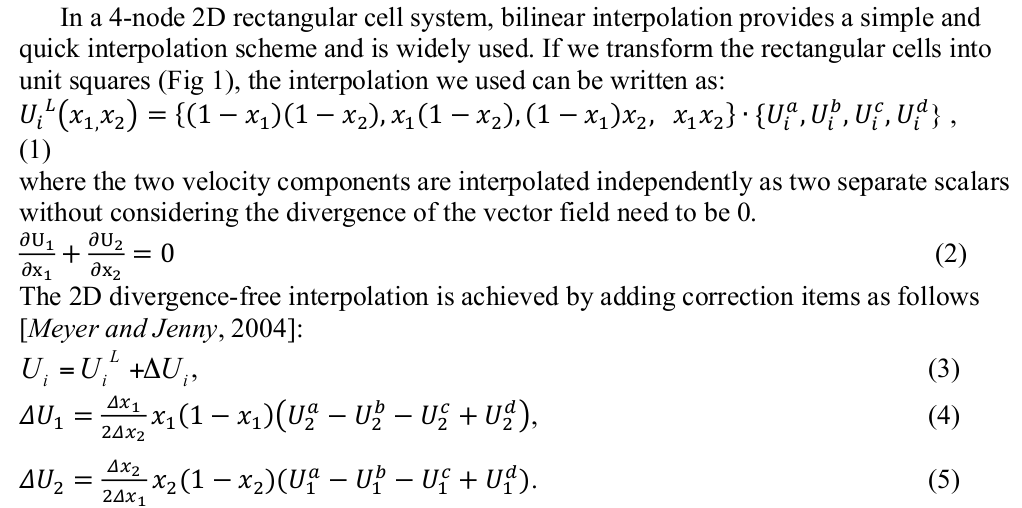
\includegraphics[width=12cm]{images/cvi/wang15_b}}\\
{\captionfont Taken from the supplementary material of Wang \etal (2015).}
\end{center}
Since basis functions must be 1 on their node, then the numbering must be as follows:
\begin{verbatim}
c--d            4--3
|  |     <=>    |  |
a--b            1--2
\end{verbatim}
Setting $\Delta x_1=\Delta x_2=1$, replacing $a$ by $1$, $b$ by 2, 
$c$ by 4 and $d$ by 3, $x_1$ by $r'$ and $x_2$ by $s'$, $U_1$ by $u$
and $U_2$ by $v$, we arrive at 
(in order to render the notations a bit lighter I have set $U=U_1$ and $V=U_2$)
\begin{eqnarray}
\Delta U &=& \frac12 r'(1-r')(v_1-v_2-v_4+v_3) = \frac12 r'(1-r')(4v_{14}-4v_{23}) \nn\\
\Delta V &=& \frac12 s'(1-s')(u_1-u_2-u_4+u_3) = \frac12 s'(1-s')(4u_{12}+4u_{34}) \nn
\end{eqnarray}
Since $r=2r'-1$ and $s=2s'-1$ then we find that 
\begin{eqnarray}
\Delta U &=& \frac12 (1-r^2)(v_{14}-v_{23}) \nn\\
\Delta V &=& \frac12 (1-s^2)(u_{12}+u_{34})
\end{eqnarray}
which is Eq.~\eqref{eq:cvi_corr1}. In the case of the reference element then 
my velocity corrections are identical to theirs.

Let us look at the equations of the figure above. 
Since the authors state that they ``transform the rectangular cells into unit squares'' 
we do away with $\Delta x_1 = \Delta x_2 = 1$. Eqs. 3 and 1 together yield:
\begin{eqnarray}
U&=&(1-x_1)(1-x_2) U^a+x_1(1-x_2)U^b + (1-x_1)x_2 U^c + x_1x_2 U^d
+ \frac12 x_1(1-x_1)(V^a-V^b-V^c+V^d) \nn\\
V&=&(1-x_1)(1-x_2) V^a+x_1(1-x_2)V^b + (1-x_1)x_2 V^c + x_1x_2 V^d
+ \frac12 x_2(1-x_2)(U^a-U^b-U^c+U^d) \nn
\end{eqnarray}
Then 
\begin{eqnarray}
\frac{\partial U}{\partial x_1} 
&=& -(1-x_2) U^a+(1-x_2)U^b -x_2 U^c + x_2 U^d + \frac12 (1-2x_1)(V^a-V^b-V^c+V^d) \nn\\
\frac{\partial V}{\partial x_2}
&=& -(1-x_1) V^a - x_1V^b + (1-x_1) V^c + x_1 V^d + \frac12 (1-2x_2)(U^a-U^b-U^c+U^d) \nn
\end{eqnarray}
So 
\begin{eqnarray}
\frac{\partial U}{\partial x_1} \! + \! \frac{\partial V}{\partial x_2} 
&=&
-(1-x_2) U^a+(1-x_2)U^b -x_2 U^c + x_2 U^d + \frac12 (1-2x_1)(V^a-V^b-V^c+V^d) \nonumber\\
&&-(1-x_1) V^a - x_1V^b + (1-x_1) V^c + x_1 V^d + \frac12 (1-2x_2)(U^a-U^b-U^c+U^d) \nonumber\\
&=& -U^a + U^b + x_2(U^a-U^b-U^c+U^d) + \frac12 (V^a-V^b-V^c+V^d)
-x_1 (V^a-V^b-V^c+V^d) \nonumber\\
&& -V^a+V^c + x_1(V^a-V^b-V^c+V^d) + \frac12 (U^a-U^b-U^c+U^d)
-x_2 (U^a-U^b-U^c+U^d) \nonumber\\
&=& -U^a + U^b  + \frac12 (V^a-V^b-V^c+V^d)
 -V^a+V^c  + \frac12 (U^a-U^b-U^c+U^d) \nonumber\\
 &\neq & 0
\end{eqnarray}
Unfortunately, the authors seem to be under the impression that 
this quantity is zero since they talk of ``2D divergence-free interpolation'' 
and ``the divergence of the vector field need to be
zero''. Their own equations prove that this is not the case.


%-----------------------------------------------------------------
\subsubsection{In 3D with $Q_1$ basis functions - Naive approach}

Let us start directly in reduced coordinates $(r,s,t)\in [-1:1]^3$:
\begin{eqnarray}
u^h(r,s,t)&=&\sum_i \bN_i(r,s,t) u_i\nn\\
v^h(r,s,t)&=&\sum_i \bN_i(r,s,t) v_i\nn\\
w^h(r,s,t)&=&\sum_i \bN_i(r,s,t) w_i\nn
\end{eqnarray}
with
\begin{eqnarray}
\bN_1&=&\frac{1}{8} (1-r)(1-s)(1-t) \nonumber\\ 
\bN_2&=&\frac{1}{8} (1+r)(1-s)(1-t) \nonumber\\ 
\bN_3&=&\frac{1}{8} (1+r)(1+s)(1-t) \nonumber\\ 
\bN_4&=&\frac{1}{8} (1-r)(1+s)(1-t) \nonumber\\ 
\bN_5&=&\frac{1}{8} (1-r)(1-s)(1+t) \nonumber\\ 
\bN_6&=&\frac{1}{8} (1+r)(1-s)(1+t) \nonumber\\ 
\bN_7&=&\frac{1}{8} (1+r)(1+s)(1+t) \nonumber\\ 
\bN_8&=&\frac{1}{8} (1-r)(1+s)(1+t) \nn
\end{eqnarray}
The incompressibility constraint imposes:
\[
\frac{\partial u^h}{\partial r}+
\frac{\partial v^h}{\partial s}+
\frac{\partial w^h}{\partial t}=0
=
\sum_i \left(  
\frac{\partial \bN_i}{\partial r} u_i+
\frac{\partial \bN_i}{\partial s} v_i+
\frac{\partial \bN_i}{\partial t} w_i
\right)
=0
\]
However, once again it is trivial to verify that the incompressibility
condition is not and can not be verified for all values of
$r,s,t \in [-1,1]^3$.

It would then make sense to think of a corrective term to the interpolation
which would add just enough degrees of freedoms so as to insure an exact
incompressibility in the element.
Let us then write:
\begin{eqnarray}
u^h(r,s,t)&=&\sum_i \bN_i(r,s,t) u_i + (a s + b t +c)(1-r)(1+r) \nn\\
v^h(r,s,t)&=&\sum_i \bN_i(r,s,t) v_i + (d r + e t +f)(1-s)(1+s) \nn\\
w^h(r,s,t)&=&\sum_i \bN_i(r,s,t) w_i + (g r + h s +i)(1-t)(1+t) \nn
\end{eqnarray}
We thereby make sure that the corrections are zero on the edges 
so that velocity remains continuous from one element to another.
In this case,
\begin{eqnarray}
\frac{\partial u^h}{\partial r}&=&\sum_i \frac{\partial \bN_i}{\partial r} u_i + (a s + b t +c)(-2r)\nn\\
\frac{\partial v^h}{\partial s}&=&\sum_i \frac{\partial \bN_i}{\partial s} v_i + (d r + e t +f)(-2s)\nn\\
\frac{\partial w^h}{\partial t}&=&\sum_i \frac{\partial \bN_i}{\partial t} w_i + (g r + h s +i)(-2t)\nn
\end{eqnarray}
We have introduced 9 coefficients  $(a,b,c,d,e,f,g,h,i)$ which remain to be determined.
The incompressibility condition is now:
\[
\sum_i \left(  
\frac{\partial \bN_i}{\partial r} u_i+
\frac{\partial \bN_i}{\partial s} v_i+
\frac{\partial \bN_i}{\partial t} w_i
\right)
+ (a s + b t +c) (-2r) + (d r + e t +f)(-2s) + (g r + h s +i)(-2t) 
=0
\]
This can be rewritten as
\[
C_0  + C_1 r + C_2 s + C_3 t + C_4 rs + C_5 st + C_6 rt = 0
\]
where the seven $C_i$ coefficients are functions of the velocities and the other coefficients.
In order for this expression to be exactly zero {\it everywhere}\footnote{By now we know 
this is not possible -- see 2D}, each $C$ coefficient has
to be independently zero.

We start with:
\begin{eqnarray}
8\sum_i \frac{\partial \bN_i}{\partial r} u_i 
&=& (1-s)(1-t)(u_2-u_1)
+ (1+s)(1-t)(u_3-u_4)
+ (1-s)(1+t)(u_6-u_5)
+ (1+s)(1+t)(u_7-u_8) \nn\\
8\sum_i \frac{\partial \bN_i}{\partial s} v_i 
&=& (1-r)(1-t)(v_4-v_1)
+ (1+r)(1-t)(v_3-v_2)
+ (1-r)(1+t)(v_8-v_5)
+ (1+r)(1+t)(v_7-v_6) \nn\\
8\sum_i \frac{\partial \bN_i}{\partial t} w_i 
&=& (1-r)(1-s)(w_5-w_1)
+ (1+r)(1-s)(w_6-w_2)
+ (1+r)(1+s)(w_7-w_3)
+ (1-r)(1+s)(w_8-w_4) \nn
\end{eqnarray}

Let us denote $u_{ij}=(u_i-v_j)/8$ (same for $v$, $w$), so that:
\begin{eqnarray}
\sum_i \frac{\partial \bN_i}{\partial r} u_i 
&=& (1-s)(1-t)u_{21}
+ (1+s)(1-t)u_{34}
+ (1-s)(1+t)u_{65}
+ (1+s)(1+t)u_{78} \nn\\
\sum_i \frac{\partial \bN_i}{\partial s} v_i 
&=& (1-r)(1-t)v_{41}
+ (1+r)(1-t)v_{32}
+ (1-r)(1+t)v_{85}
+ (1+r)(1+t)v_{76} \nn\\
\sum_i \frac{\partial \bN_i}{\partial t} w_i 
&=& 
  (1-r)(1-s)w_{51}
+ (1+r)(1-s)w_{62}
+ (1+r)(1+s)w_{73}
+ (1-r)(1+s)w_{84} \nn
\end{eqnarray}
We finally arrive at:
\begin{eqnarray}
C_0   &(.)  &  u_{21} + u_{34} + u_{65} + u_{78} + v_{41} + v_{32} + v_{85} + v_{76} + w_{51} + w_{62} + w_{73} + w_{84} =0  \nn\\
C_1   &(r)  &  -v_{41} +v_{32} -v_{85} + v_{76} - w_{51} + w_{62} + w_{73} -w_{84} -2c =0\nn\\ 
C_2   &(s)  &  -u_{21} +u_{34} -u_{65} + u_{78} - w_{51} - w_{62} + w_{73} +w_{84} -2f =0 \nn\\ 
C_3   &(t)  &  -u_{21} -u_{34} +u_{65} + u_{78} - v_{41} - v_{32} + v_{85} +v_{76} -2i =0 \nn\\ 
C_4   &(rs) &  w_{51} -w_{62} +w_{73} - w_{84}  -2a -2d =0  \nn\\
C_5   &(st) &  u_{21} -u_{34} -u_{65} + u_{78}  -2e -2h =0  \nn\\
C_6   &(rt) &  v_{41} -v_{32} -v_{85} + v_{76}  -2b -2g =0  \nn
\end{eqnarray}

I leave $C_0$ alone but I still unfortunately end up with 6 equations and 9 unknowns $a,b,c,d,e,f,g,h$.
Coming up with additional constraints is not trivial, so I will instead further assume 
$\alpha_r=b=a$, $\alpha_s=e=d$ and $\alpha_t=h=g$, and rename 
$\beta_r=c$, $\beta_s=f$ and $\beta_t=i$ so that
I have now six unknowns $\alpha_r,\alpha_s,\alpha_t,\beta_r,\beta_s,\beta_t$ for six equations
\begin{eqnarray}
C_1   &(r)  &  -v_{41} +v_{32} -v_{85} + v_{76} - w_{51} + w_{62} + w_{73} -w_{84} -2\beta_r \nn\\ 
C_2   &(s)  &  -u_{21} +u_{34} -u_{65} + u_{78} - w_{51} - w_{62} + w_{73} +w_{84} -2\beta_s \nn\\ 
C_3   &(t)  &  -u_{21} -u_{34} +u_{65} + u_{78} - v_{41} - v_{32} + v_{85} +v_{76} -2\beta_t \nn\\ 
C_4   &(rs) &  w_{51} -w_{62} +w_{73} - w_{84}  -2\alpha_r -2\alpha_s   \nn\\
C_5   &(st) &  u_{21} -u_{34} -u_{65} + u_{78}  -2\alpha_s -2\alpha_t   \nn\\
C_6   &(rt) &  v_{41} -v_{32} -v_{85} + v_{76}  -2\alpha_r -2\alpha_t   \nn
\end{eqnarray}


This naturally yields:
\begin{eqnarray}
\beta_r
&=& \frac{1}{2} ( -v_{41} +v_{32} -v_{85} + v_{76} - w_{51} + w_{62} + w_{73} -w_{84}  ) \nn\\
&=& \frac{1}{16} (v_1-v_2+v_3-v_4+v_5-v_6+v_7-v_8  +w_1-w_2 - w_3 + w_4 - w_5 + w_6 +w_7  - w_8    )  \nn\\
\beta_s&=& \frac{1}{2} ( -u_{21} +u_{34} -u_{65} + u_{78} - w_{51} - w_{62} + w_{73} +w_{84}  ) \nn\\
&=& \frac{1}{16} (u_1-u_2+u_3-u_4+u_5-u_6+u_7-u_8  +w_1 + w_2 - w_3 - w_4 - w_5 - w_6 +w_7 + w_8   )  \nn\\
\beta_t&=& \frac{1}{2} ( -u_{21} -u_{34} +u_{65} + u_{78} - v_{41} - v_{32} + v_{85} +v_{76}   ) \nn\\
&=& \frac{1}{16} ( u_1-u_2-u_3+u_4 -u_5 + u_6 + u_7 - u_8 +v_1 +v_2 - v_3 - v_4 - v_5 - v_6 + v_7 + v_8  )  \nn
\end{eqnarray}
and we need to solve
\begin{eqnarray}
\tilde{w} -2\alpha_r -2\alpha_s&=&0\nn\\
\tilde{u} -2\alpha_s -2\alpha_t&=&0\nn\\
\tilde{v} -2\alpha_r -2\alpha_t&=&0\nn
\end{eqnarray}
where
\begin{eqnarray}
\tilde{u} 
&=& u_{21} -u_{34} -u_{65} + u_{78} 
=\frac{1}{8}(-u_1 + u_2-u_3+u_4 + u_5-u_6 + u_7-u_8  )
\nn\\
\tilde{v} 
&=& v_{41} -v_{32} -v_{85} + v_{76}
= \frac{1}{8} (-v_1 + v_2 - v_3 + v_4 + v_5 - v_6 + v_7 - v_8    )
  \nn\\ 
\tilde{w} 
&=&  w_{51} -w_{62} +w_{73} - w_{84} 
=\frac{1}{8} (-w_1+w_2-w_3+w_4 + w_5 - w_6 + w_7 -w_8  )
\nn
\end{eqnarray}
which yields:
\[
\alpha_r=\frac{1}{4} ( -\tilde{u} + \tilde{v} + \tilde{w} ) 
\quad\quad
\alpha_s=\frac{1}{4} ( \tilde{u} - \tilde{v} + \tilde{w} ) 
\quad\quad
\alpha_t=\frac{1}{4} ( \tilde{u} + \tilde{v} - \tilde{w} ) 
\]

So finally:

\begin{eqnarray}
u^h(r,s,t)&=&\sum_i \bN_i(r,s,t) u_i + [\alpha_r (s+t) +\beta_r](1-r)(1+r) \nn\\
v^h(r,s,t)&=&\sum_i \bN_i(r,s,t) v_i + [\alpha_s (r+t) +\beta_s](1-s)(1+s) \nn\\
w^h(r,s,t)&=&\sum_i \bN_i(r,s,t) w_i + [\alpha_t (r+s) +\beta_t](1-t)(1+t) \nn
\end{eqnarray}


%-------------------------------------------------------------------
\subsubsection{In 3D with $Q_1$ basis functions - better approach}

We start again from 
\[
\left(
\begin{array}{c}
\frac{\partial f}{\partial x} \\ \\
\frac{\partial f}{\partial y} \\ \\
\frac{\partial f}{\partial z} 
\end{array}
\right)
=
\tilde{\bm J} \cdot
\left(
\begin{array}{c}
\frac{\partial f}{\partial r} \\ \\
\frac{\partial f}{\partial s} \\ \\ 
\frac{\partial f}{\partial t} 
\end{array}
\right)
\]
We then postulate 
\begin{eqnarray}
u^h(r,s,t)&=&\sum_i \bN_i(r,s,t) u_i + (a s + b t +c)(1-r)(1+r) \nn\\
v^h(r,s,t)&=&\sum_i \bN_i(r,s,t) v_i + (d r + e t +f)(1-s)(1+s) \nn\\
w^h(r,s,t)&=&\sum_i \bN_i(r,s,t) w_i + (g r + h s +i)(1-t)(1+t) \nn
\end{eqnarray}
so that:
\begin{eqnarray}
\frac{\partial u}{\partial x} 
&=& \tilde{J}_{xx} \frac{\partial u^h}{\partial r} 
+\tilde{J}_{xy} \frac{\partial u}{\partial s}
+\tilde{J}_{xz} \frac{\partial u}{\partial t} \nn\\
&=&  \tilde{J}_{xx} \left[\sum_i \frac{\partial \bN_i}{\partial r} u_i + (a s + b t +c)(-2r)  \right]\! %\nn\\
+\tilde{J}_{xy} \left[\sum_i \frac{\partial \bN_i}{\partial s} u_i + a (1-r^2)  \right]\! %\nn\\
+\tilde{J}_{xz} \left[\sum_i \frac{\partial \bN_i}{\partial t} u_i + b (1-r^2)  \right]
\nn\\
\frac{\partial v}{\partial y} 
&=& \tilde{J}_{yx} \frac{\partial v^h}{\partial r} 
+\tilde{J}_{yy} \frac{\partial v}{\partial s}
+\tilde{J}_{yz} \frac{\partial v}{\partial t} \nn\\
&=&  \tilde{J}_{yx} \left[\sum_i \frac{\partial \bN_i}{\partial r} v_i + d (1-s^2)  \right]\!
+\tilde{J}_{yy} \left[\sum_i \frac{\partial \bN_i}{\partial s} v_i + (d r + e t +f)(-2s) \right]\!
+\tilde{J}_{yz} \left[\sum_i \frac{\partial \bN_i}{\partial t} v_i + e (1-s^2)  \right] 
\nn\\
\frac{\partial w}{\partial z} 
&=& \tilde{J}_{zx} \frac{\partial w^h}{\partial r} 
+\tilde{J}_{zy} \frac{\partial w}{\partial s}
+\tilde{J}_{zz} \frac{\partial w}{\partial t} \nn\\
&=&  \tilde{J}_{zx} \left[\sum_i \frac{\partial \bN_i}{\partial r} w_i + g (1-t^2)  \right]\! 
+\tilde{J}_{zy} \left[\sum_i \frac{\partial \bN_i}{\partial s} w_i + h (1-t^2) \right] \! 
+\tilde{J}_{zz} \left[\sum_i \frac{\partial \bN_i}{\partial t} w_i + (g r + h s +i)(-2t)  \right] \nn
\end{eqnarray}

where for any function $f$:
\begin{eqnarray}
\sum_i
\frac{\partial \bN_i}{\partial r} f_i 
%&=&
% (1-s)(1-t)(f_{2}-f_1)
%+(1-s)(1+t)(f_{6}-f_5)
%+(1+s)(1-t)(f_{3}-f_4)
%+(1+s)(1+t)(f_{7}-f_8) \nn\\
&=&
 (1-s)(1-t)f_{21}
+(1-s)(1+t)f_{65}
+(1+s)(1-t)f_{34}
+(1+s)(1+t)f_{78} 
\nn\\
&=& ( f_{21}+f_{65}+f_{34}+f_{78}) \nn\\
&+& (-f_{21}-f_{65}+f_{34}+f_{78})s \nn\\
&+& (-f_{21}+f_{65}-f_{34}+f_{78})t \nn\\
&+& ( f_{21}-f_{65}-f_{34}+f_{78})st 
\nn\\
&=& f_{r1} + f_{r2}s + f_{r3}t + f_{r4} st \nn\\ 
\sum_i
\frac{\partial \bN_i}{\partial s} f_i 
%&=&
% (1-r)(1-t)(f_4-f_1)
%+(1+r)(1-t)(f_3-f_2)
%+(1-r)(1+t)(f_8-f_5)
%+(1+r)(1+t)(f_7-f_6) \nn\\
&=&
 (1-r)(1-t)f_{41}
+(1+r)(1-t)f_{32}
+(1-r)(1+t)f_{85}
+(1+r)(1+t)f_{76} \nn\\
&=&
   ( f_{41}+f_{32}+f_{85}+f_{76})  \nn\\
&+&(-f_{41}+f_{32}-f_{85}+f_{76})r \nn\\
&+&(-f_{41}-f_{32}+f_{85}+f_{76})t \nn\\
&+&( f_{41}-f_{32}-f_{85}+f_{76})rt
\nn\\
&=& f_{s1} + f_{s2}r + f_{s3}t + f_{s4} rt \nn\\ 
\sum_i
\frac{\partial \bN_i}{\partial t} f_i 
&=&
 (1-r)(1-s)f_{51}
+(1+r)(1-s)f_{62}
+(1+r)(1+s)f_{73}
+(1-r)(1+s)f_{84} \nn\\
&=&( f_{51}+f_{62}+f_{73}+f_{84}) \nn\\ 
&+&(-f_{51}+f_{62}+f_{73}-f_{84})r\nn\\
&+&(-f_{51}-f_{62}+f_{73}+f_{84})s\nn\\
&+&( f_{51}-f_{62}+f_{73}-f_{84})rs
\nn\\
&=& f_{t1} + f_{t2}r + f_{t3}s + f_{t4} rs \nn
\end{eqnarray}
The velocity divergence is then 
\[
 \frac{\partial u}{\partial x} 
+\frac{\partial v}{\partial y} 
+\frac{\partial w}{\partial z} 
= C_0 +C_1 r + C_2 s + C_3 t + C_4 rs + C_5 st + C_6 rt + C_7r^2 + C_8 s^2 + C_9 t ^2 =0
\]
with:
\begin{eqnarray}
C_0 &=&
\tilde{J}_{xx} u_{r1} + \tilde{J}_{xy} u_{s1} + \tilde{J}_{xz} u_{t1} + 
\tilde{J}_{yx} v_{r1} + \tilde{J}_{yy} v_{s1} + \tilde{J}_{yz} v_{t1} + 
\tilde{J}_{zx} w_{r1} + \tilde{J}_{zy} w_{s1} + \tilde{J}_{zz} w_{t1} \nn\\
&+&\tilde{J}_{xy} a+\tilde{J}_{xz} b + \tilde{J}_{yx} d + \tilde{J}_{yz} e + \tilde{J}_{zx} g + \tilde{J}_{zy} h \nn\\
C_1 &=& 
J_{xy} u_{s2} + J_{xz} u_{t2} + 
J_{yy} v_{s2} + J_{yz} v_{t2} + 
J_{zy} w_{s2} + J_{zz} w_{t2} -J_{xx} 2c \nn \\ % r
C_2 &=&
J_{xx} u_{r2} + J_{xz} u_{t3} +
J_{yx} v_{r2} + J_{yz} v_{t3} +
J_{zx} w_{r2} + J_{zz} w_{t3} -J_{yy} 2f \nn\\ % s 
C_3 &=&
J_{xx} u_{r3} + J_{xy} u_{s3} +
J_{yx} v_{r3} + J_{yy} v_{s3} +
J_{zy} w_{r3} + J_{zy} w_{s3} -J_{zz} 2i \nn\\ % t 
C_4 &=& J_{xz} u_{t4} + J_{yz} v_{t4} + J_{zz} w_{t4} -J_{xx} 2a - J_{yy} 2d  \nn\\ % rs
C_5 &=& J_{xx} u_{r4} + J_{yx} v_{r4} + J_{zx} w_{r4} -J_{yy} 2e - J_{zz} 2h  \nn\\ % st
C_6 &=& J_{xy} u_{s4} + J_{yy} v_{s4} + J_{zy} w_{s4} -J_{xx} 2b - J_{zz} 2g  \nn\\ % rt
C_7 &=& - \tilde{J}_{xy} a - \tilde{J}_{xz} b  \nn\\ % r^2 
C_8 &=& - \tilde{J}_{yx} d - \tilde{J}_{yz} e  \nn\\ % s^2 
C_9 &=& - \tilde{J}_{zx} g - \tilde{J}_{zy} h  \nn   % t^2
\end{eqnarray}
It is then trivial to obtain $c,f,i$. 
Concerning $a,b,d,e,g,h$ we are left with 6 equations for 6 unknowns, which can be cast as follows:
\[
\left(
\begin{array}{cccccc}
J_{xx} & & J_{yy} & & & \\
 & & & J_{yy} & &  J_{zz}\\ 
 & J_{xx} & & & J_{zz} & \\ 
J_{xy} &  J_{xz} & & & & \\ 
 & & J_{yx} & J_{yz} & \\ 
 & & & & -J_{zx} & J_{zy} \\ 
\end{array}
\right)
\left(
\begin{array}{c}
a \\b\\ d\\ e\\ g\\ h
\end{array}
\right)
=
\frac{1}{2}
\left(
\begin{array}{c}
 J_{xz} u_{t4} + J_{yz} v_{t4} + J_{zz} w_{t4} \\
 J_{xx} u_{r4} + J_{yx} v_{r4} + J_{zx} w_{r4} \\
 J_{xy} u_{s4} + J_{yy} v_{s4} + J_{zy} w_{s4} \\
 0 \\ 0 \\  0
\end{array}
\right)
\]
In the case of a regular grid with nodes aligned with the x,y,z axis, this 
system is indefinite as $J_{xy}=J_{yx}=J_{xz}=...=0$.

We can approach it simply:
from the last three equations we have 
\[
b=-\frac{J_{xy}}{J_{xz}} a \quad\quad
e=-\frac{J_{yx}}{J_{yz}} d \quad\quad
h=-\frac{J_{zx}}{J_{zy}} g
\]
The equations involving $C_4$, $C_5$, $C_6$ become:
\begin{eqnarray}
C_4 &=& J_{xz} u_{t4} + J_{yz} v_{t4} + J_{zz} w_{t4} -J_{xx} 2a - J_{yy} 2d  \nn\\ % rs
C_5 &=& J_{xx} u_{r4} + J_{yx} v_{r4} + J_{zx} w_{r4} +2J_{yy} \frac{J_{yx}}{J_{yz}} d + 2J_{zz} \frac{J_{zx}}{J_{zy}}  \nn\\ % st
C_6 &=& J_{xy} u_{s4} + J_{yy} v_{s4} + J_{zy} w_{s4} +2J_{xx} \frac{J_{xy}}{J_{xz}} a - J_{zz} 2g  \nn\\ % rt
\end{eqnarray}

%-------------------------------------------------------------------
\subsubsection{Comparison with Wang \etal (2015) for 3D}

The following is taken from the supplementary material of Wang \etal (2015):
\begin{center}
\fbox{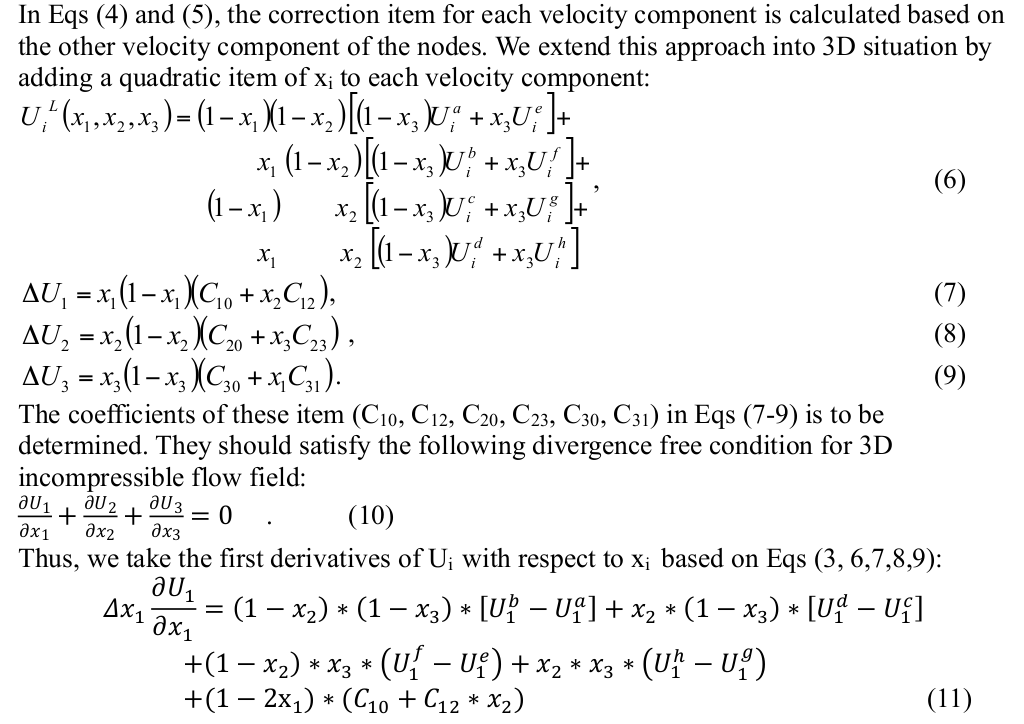
\includegraphics[width=11cm]{images/cvi/wang15_c}}\\
\fbox{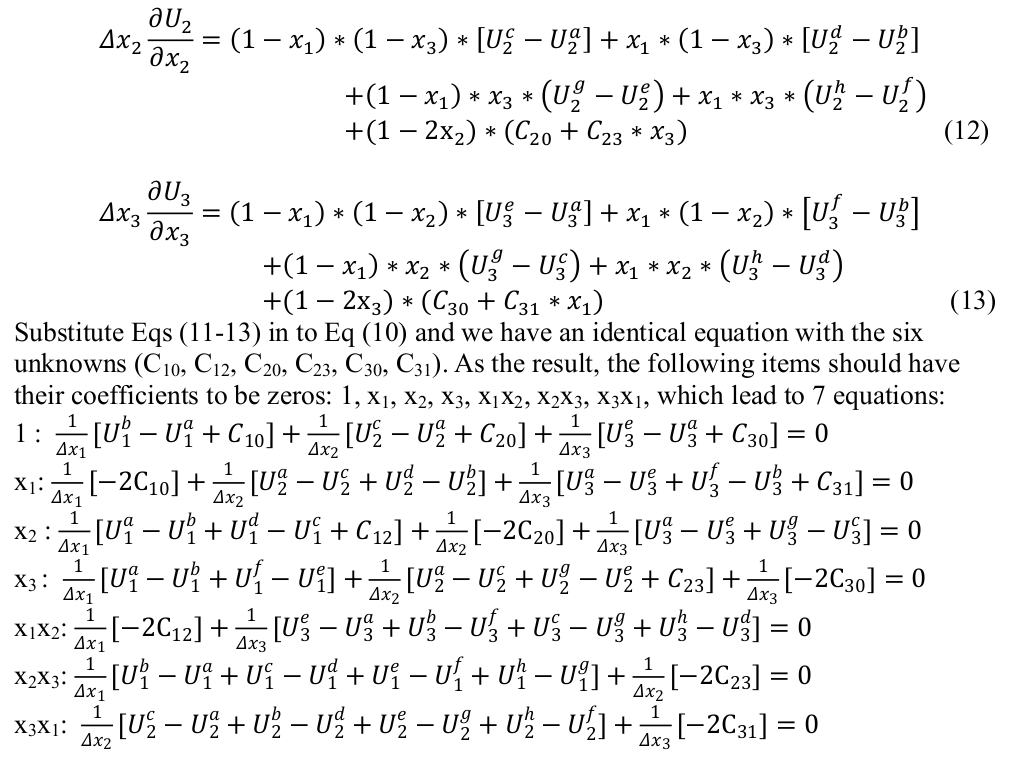
\includegraphics[width=11cm]{images/cvi/wang15_d}}\\
\fbox{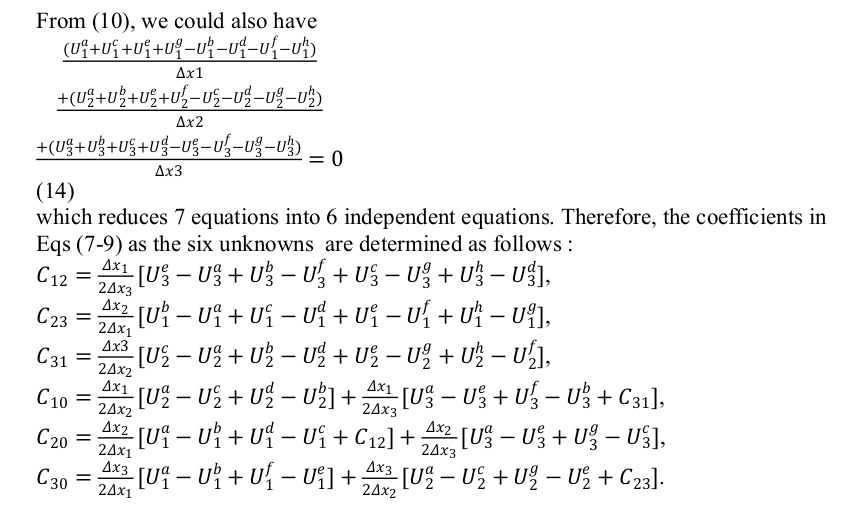
\includegraphics[width=11cm]{images/cvi/wang15_e}}\\
{\captionfont Taken from the supplementary material of Wang \etal (2015).}
\end{center}
In my opinion, it is quite unbelievable that such a document was accepted for publication
(even as supplementary material). 
There is not much justification for why their equation 7 only contains $x_2$ and not also 
$x_3$, same for the other two equations. 
Rather surprising is also the fact that although equations 3,6,7,8,9 do not contain 
any $\Delta x_{\{1,2,3\}}$term  then equations 11,12,13 do feature them. 
Nevertheless, we must make sense of this mess. 

Since the authors state that they ``transform the rectangular cells into unit squares'' 
I do away with $\Delta x_1 = \Delta x_2 = \Delta x_3 =1$ altogether. 
Also, $U_1,U_2,U_3$ have become $U,V,W$.

The polynomial representation of $U,V,W$ on the element including the correction factors is
\begin{eqnarray}
U 
&=&(1-x_1)(1-x_2)(1-x_3) U^a 
+(1-x_1)(1-x_2)x_3 U^e \nonumber\\
&+&x_1(1-x_2)(1-x_3) U^b 
+x_1(1-x_2)x_3 U^f \nonumber\\
&+&(1-x_1)x_2(1-x_3) U^c 
+(1-x_1)x_2 x_3 U^g \nonumber\\
&+&x_1 x_2(1-x_3) U^d 
+ x_1 x_2 x_3 U^h \nonumber\\
&+& x_1(1-x_1)(C_{10}+x_2 C_{12})\\
V 
&=&(1-x_1)(1-x_2)(1-x_3) V^a 
+(1-x_1)(1-x_2)x_3 V^e \nonumber\\
&+&x_1(1-x_2)(1-x_3) V^b
+x_1(1-x_2)x_3 V^f \nonumber\\
&+&(1-x_1)x_2(1-x_3) V^c 
+(1-x_1)x_2 x_3 V^g \nonumber\\
&+&x_1 x_2(1-x_3) V^d 
+x_1 x_2 x_3 V^h \nonumber\\
&+& x_2(1-x_2)(C_{20}+x_3 C_{23})\\
W 
&=&(1-x_1)(1-x_2)(1-x_3) W^a 
+(1-x_1)(1-x_2)x_3 W^e \nonumber\\
&+&x_1(1-x_2)(1-x_3) W^b
+x_1(1-x_2)x_3 W^f \nonumber\\
&+&(1-x_1)x_2(1-x_3) W^c 
+(1-x_1)x_2 x_3 W^g \nonumber\\
&+&x_1 x_2(1-x_3) W^d 
+ x_1 x_2 x_3 W^h \nonumber\\
&+& x_3(1-x_3)(C_{30}+x_1 C_{31})
\end{eqnarray}


Then 
\begin{eqnarray}
\frac{\partial U}{\partial x_1}  
&=&-(1-x_2)(1-x_3) U^a 
-(1-x_2)x_3 U^e 
+(1-x_2)(1-x_3) U^b
+(1-x_2)x_3 U^f \nonumber\\
&+&-x_2(1-x_3) U^c 
-x_2 x_3 U^g 
+ x_2(1-x_3) U^d 
+  x_2 x_3 U^h \nonumber\\
&+& (1-2x_1)(C_{10}+x_2 C_{12})
\\
\frac{\partial V}{\partial x_2}
&=&-(1-x_1)(1-x_3) V^a 
-(1-x_1)x_3 V^e 
-x_1(1-x_3) V^b
-x_1x_3 V^f \nonumber\\
&+&(1-x_1)(1-x_3) V^c
+(1-x_1) x_3 V^g 
+x_1 (1-x_3) V^d 
+x_1  x_3 V^h \nonumber\\
&+& (1-2x_2)(C_{20}+x_3 C_{23})
\\
\frac{\partial W}{\partial x_3} 
&=&-(1-x_1)(1-x_2) W^a 
+(1-x_1)(1-x_2) W^e 
-x_1(1-x_2) W^b
+x_1(1-x_2) W^f \nonumber\\
&-&(1-x_1)x_2 W^c 
+(1-x_1)x_2  W^g 
-x_1 x_2 W^d 
+ x_1 x_2  W^h \nonumber\\
&+& (1-2x_3)(C_{30}+x_1 C_{31})
\end{eqnarray}
So the velocity divergence can be written 
\begin{eqnarray}
\frac{\partial U}{\partial x_1}
+
\frac{\partial V}{\partial x_2} 
+
\frac{\partial W}{\partial x_3} 
= A + Bx_1 + Cx_2 + Dx_3 + E x_1x_2 + Fx_2x_3 + G x_3x_1
\end{eqnarray}
with
\begin{eqnarray}
A &=& -U^a + U^b  + C_{10} -V^a + V^c + C_{20} -W^a + W^e + C_{30}
\\
B &=& -2 C_{10} + V^a -V^b -V^c +V^d  + W^a -W^e -W^b +W^f +C_{31}
\\
C &=& U^a -U^b -U^c +U^d + C_{12} -2 C_{20} +W^a -W^e -W^c +W^g
\\
D &=& U^a -U^e -U^b +U^f + V^a -V^e -V^c +V^g + C_{23} -2C_{30}
\\
E &=& -2C_{12}  -W^a +W^e +W^b -W^f + W^c -W^g -W^d +W^h
\\
F &=& -U^a +U^e +U^b -U^f +U^c -U^g -U^d +U^h   -2C_{23}
\\
G &=&   -V^a +V^e +V^b -V^f +V^c -V^g -V^d + V^h -2C_{31}
\end{eqnarray}
A term by term comparison of these equations shows that these are identical to the 
7 equations in the supplementary material between Eq.~13 and Eq.~14 (why are these not 
numbered in the supplementary material?).

Ideally we wish to have all 7 coefficients $A$ to $G$ equal to zero. 
This leaves us with 7 equations involving 6 unknowns.
In other words the system is over constrained and cannot be solved. 
However the authors seem to interprete this in the exact opposite way by offering 
yet one more constraint (Eq.~14) which a) is irrelevant b) is not justified (it is 
indeed related to Eq.~10 but only by taking all $C_{ij}$ coefficients equal to zero and expressed 
for $x_1=x_2=x_3=1/2$). Funny enough, that constraint of Eq.~14 is not used further... 

From $E=0,F=0,G=0$ we get:
\begin{eqnarray}
C_{12} &=& \frac12 ( -W^a +W^e +W^b -W^f + W^c -W^g -W^d +W^h )\\
C_{23} &=& \frac12 (-U^a +U^e +U^b -U^f +U^c -U^g -U^d +U^h  ) \\
C_{31} &=& \frac12 ( -V^a +V^e +V^b -V^f +V^c -V^g -V^d + V^h )
\end{eqnarray}
and from $B=0,C=0,D=0$ we get 
\begin{eqnarray}
C_{10} &=& \frac12 ( V^a -V^b -V^c +V^d  + W^a -W^e -W^b +W^f +C_{31} ) \\
C_{20} &=& \frac12 ( U^a -U^b -U^c +U^d + C_{12} +W^a -W^e -W^c +W^g ) \\
C_{30} &=& \frac12 (U^a -U^e -U^b +U^f + V^a -V^e -V^c +V^g + C_{23} )
\end{eqnarray}
These 6 expressions are identical to the ones in the paper. 
However, let us now turn to $A$:
\begin{eqnarray}
A 
&=& -U^a + U^b  + C_{10} -V^a + V^c + C_{20} -W^a + W^e + C_{30} \\
&=& -U^a + U^b +\frac12 ( V^a -V^b -V^c +V^d  + W^a -W^e -W^b +W^f +C_{31} ) \\
&&-V^a + V^c + \frac12 ( U^a -U^b -U^c +U^d + C_{12} +W^a -W^e -W^c +W^g ) \\
&&-W^a + W^e + \frac12 (U^a -U^e -U^b +U^f + V^a -V^e -V^c +V^g + C_{23} ) \\
&=& -U^a + U^b +\frac12 ( V^a -V^b -V^c +V^d  + W^a -W^e -W^b +W^f ) \\
&&+\frac12 \frac12 ( -V^a +V^e +V^b -V^f +V^c -V^g -V^d + V^h ) \\
&&-V^a + V^c + \frac12 ( U^a -U^b -U^c +U^d  +W^a -W^e -W^c +W^g ) \\
&&+\frac12 \frac12 ( -W^a +W^e +W^b -W^f + W^c -W^g -W^d +W^h ) \\
&&-W^a + W^e + \frac12 (U^a -U^e -U^b +U^f + V^a -V^e -V^c +V^g +  ) \\ 
&& +\frac12 \frac12 (-U^a +U^e +U^b -U^f +U^c -U^g -U^d +U^h  ) \\
&\neq& 0
\end{eqnarray}
(easy to prove: for example $W^h$ appears only once)

Once again, we find that the divergence is not identically zero in the element, thereby refuting the 
statement ``Adding these corrections does not improve the order of accuracy of 
the interpolation (it remains a second-order accurate scheme), but they ensure 
a divergence-free velocity field over the cell'' on page 3 of the article. 
Their entire paper is based on a false premise.

%------------------------------------------------------------------------
\subsubsection{In 2D with $P_1$ basis functions - what about triangles?}


The reference linear element is: 
\begin{verbatim}
s
|
3
|\
|  \
|    \
1-----2 ->r
\end{verbatim}

The basis functions are 
\begin{eqnarray}
\bN_1(r,s) &=& 1-r-s \nn\\
\bN_2(r,s) &=& r \nn\\
\bN_3(r,s) &=& s 
\end{eqnarray}
and the velocity vector is $\vec\upnu=(u,v)$. 
Its representation inside the element is 
\begin{eqnarray}
u^h(r,s)&=&\sum_i \bN_i(r,s) u_i \nn\\
v^h(r,s)&=&\sum_i \bN_i(r,s) v_i \nn
\end{eqnarray}
and the velocity divergence in the element is given by
\[
(\vec\nabla\cdot\vec\upnu)^h = 
\frac{\partial u^h}{\partial r}
+
\frac{\partial v^h}{\partial s}
=(-u_1+u_2)+(-v_1+v_3)
\]
which is evidently not zero everywhere in the element.
There is however a fundamental difference with regards to quadrilaterals
for which the same quantity still contains $r$ and $s$ terms which 
opens the door to a correction in order to cancel them.
In this case, not so much: this term is exactly the one
we could not get rid off for quads!

The following consists of a few misguided attempts at designing a 
CVI scheme for triangles despite the above observation.

%_______________________________
\paragraph{approach 1}
As we have seen before the CVI approach consists in adding polynomial 
terms to the expressions of $u^h$ and $v^h$.
In what follows I assume that the additional terms are of the form 
(I here use only two basis functions per line, similarly to the quadrilateral counterpart):
\begin{eqnarray}
u^h(r,s)&=&\sum_i N_i(r,s) u_i + f(r,s) r(1-r-s) \\
v^h(r,s)&=&\sum_i N_i(r,s) v_i + g(r,s) s(1-r-s) 
\end{eqnarray}
Note that we thereby ensure that $u$ is continuous across edges, and so is $v$.

The velocity divergence requirement is then
\begin{eqnarray}
0=\vec\nabla\cdot\vec\upnu_h 
&=& 
  -u_1+u_2 + \partial_r f r(1-r-s) + f(r,s)(1-2r-s) \\
&&-v_1+v_3 + \partial_s g s(1-r-s) + g(r,s)(1-2s-r)
\end{eqnarray}

\begin{itemize}
\item
We start simple and postulate $f(r,s)=a$, $g(r,s)=b$, so then 
\begin{eqnarray}
0=\vec\nabla\cdot\vec\upnu_h 
&=&   -u_1+u_2 +  a(1-2r-s) -v_1+v_3 +  b(1-2s-r) \\
&=&  (-u_1+u_2-v_1+v_3 +a +b ) + (-2a-b)r + (-a-2b)s
\end{eqnarray}
It is impossible to find $a$ and $b$ such that this expression is zero everywhere inside the element.

\item
We then turn to linear functions and postulate then $f(r,s)=a+br+cs$, $g(r,s)=d+er+fs$, so  
\begin{eqnarray}
0=\vec\nabla\cdot\vec\upnu_h 
&=& -u_1+u_2 + \partial_r f r(1-r-s) + f(r,s)(1-2r-s) \nn\\
&&  -v_1+v_3 + \partial_s g s(1-r-s) + g(r,s)(1-2s-r) \nn\\
&=& -u_1+u_2 + b r(1-r-s) + (a+br+cs) (1-2r-s) \nn\\
&&  -v_1+v_3 + f s(1-r-s) + (d+er+fs)(1-2s-r) \nn\\
&=& -u_1+u_2  -v_1+v_3 + a + d \nn\\
&& +(b-2a+b-d+e)r \nn\\
&& +(f-a+c-2d+f)s \nn\\
&& +(-b-2b-e)r^2 \nn\\
&& +(-f-c-2f)s^2 \nn\\
&& +(-b-f-b-2c-2e-f)rs \nn\\
&=& -u_1+u_2  -v_1+v_3 + a + d \nn\\
&& +(2b-2a-d+e)r \nn\\
&& +(2f-a+c-2d)s \nn\\
&& +(-3b-e)r^2 \nn\\
&& +(-3f-c)s^2 \nn\\
&& +(-2b-2f-2c-2e)rs  \nn
\end{eqnarray}
Immediately $e=-3b$ and $c=-3f$. Inserting these in the last line yields
$-2b-2f-2c-2e=-2b-2f+6f+6b=4b+4f=0$, i.e. $b=-f$.
Inserting these in the remaining lines:
\begin{eqnarray}
a+d &=& u_1-u_2  +v_1-v_3 \nn\\
2b-2a-d+(-3b) &=& 0 \nn\\
2(-b)-a+(3b)-2d &=& 0 \nn
\end{eqnarray}
or,
\begin{eqnarray}
a+d &=& u_1-u_2  +v_1-v_3 \nn\\
-2a-b-d &=& 0 \nn\\
-a + b-2d &=& 0 \nn
\end{eqnarray}
or, 
\[
\left(
\begin{array}{ccc}
1 &0 & 1 \\
-2 & -1 & -1 \\
-1 & 1 & -2 
\end{array}
\right)
\cdot
\left(
\begin{array}{c}
a \\ b  \\d 
\end{array}
\right)
=
\left(
\begin{array}{c}
u_1-u_2+v_1-v_3 \\
0 \\ 0 
\end{array}
\right)
\]
Determinant= 3 -2 -1 = 0. Matrix is singular ... !! 

\item We now try bilinear functions and 
postulate $f(r,s)=a+br+cs+hrs$, $g(r,s)=d+er+fs+krs$, so then 

\begin{eqnarray}
0=\vec\nabla\cdot\vec\upnu_h 
&=& -u_1+u_2 + \partial_r f r(1-r-s) + f(r,s)(1-2r-s) \nn\\
&&  -v_1+v_3 + \partial_s g s(1-r-s) + g(r,s)(1-2s-r) \nn\\
&=& -u_1+u_2 + (b+hs) r(1-r-s) + (a+br+cs+hrs) (1-2r-s) \nn\\
&&  -v_1+v_3 + (f+kr) s(1-r-s) + (d+er+fs+krs)(1-2s-r) \nn\\
&=& -u_1+u_2  -v_1+v_3 + a + d \nn\\
&& +(b-2a+b-d+e)r \nn\\
&& +(f-a+c-2d+f)s \nn\\
&& +(-b-2b-e)r^2 \nn\\
&& +(-f-c-2f)s^2 \nn\\
&& +(-b-f-b-2c-2e-f+2h+2k)rs \nn\\
&& +(-h-k-2k-h)rs^2 \nn\\
&& +(-h-k-2h-k)r^2s \nn\\
&=& -u_1+u_2  -v_1+v_3 + a + d \nn\\
&& +(b-2a+b-d+e)r \nn\\
&& +(f-a+c-2d+f)s \nn\\
&& +(-3b-e)r^2 \nn\\
&& +(-3f-c)s^2 \nn\\
&& +(-2b-2f-2c-2e+2h+2k)rs \nn\\
&& +(-2h-3k)rs^2 \nn\\
&& +(-3h-2k)r^2s 
\end{eqnarray}
Immediately we see that the last 2 lines yield $k=h=0$ which are the coefficients 
in front of the new terms (with regards to linear $f$ and $g$). This is a dead end too. 

I {\it could} keep adding high order terms but I suspect it is a doomed effort 
and even if it would work, the cost would be prohibitive.

\end{itemize}


%_______________________________
\paragraph{approach 2} This time I include all three basis functions $r$ , $s$ and $1-r-s$, 
not just two. Then

\begin{eqnarray}
u^h(r,s)&=&\sum_i N_i(r,s) u_i + f(r,s) rs(1-r-s) \\
v^h(r,s)&=&\sum_i N_i(r,s) v_i + g(r,s) rs(1-r-s) 
\end{eqnarray}

\begin{eqnarray}
0=\vec\nabla\cdot\vec\upnu^h
&=& 
  -u_1+u_2 + \partial_r f \; rs(1-r-s) + f(r,s)s(1-2r-s) \\
&&-v_1+v_3 + \partial_s g \; rs(1-r-s) + g(r,s)r(1-2s-r)
\end{eqnarray}


We postulate $f(r,s)=a$, $g(r,s)=b$, so then 
\begin{eqnarray}
0=\vec\nabla\cdot\vec\upnu^h 
&=&   -u_1+u_2 +  as(1-2r-s) -v_1+v_3 +  br(1-2s-r) \\
&=&  (-u_1+u_2 -v_1+v_3) + ...
\end{eqnarray}
This is also a dead end and this will not change with high order 
terms in $f$ and $g$. Because of the presence of all three 
basis functions in the additional terms we see that no 
coefficient will enter the parenthesis above and therefore it is doomed. 


%_______________________________
\paragraph{approach 3} 

We start from
\[
\left(
\begin{array}{c}
\frac{\partial u}{\partial x} \\ \\
\frac{\partial u}{\partial y} 
\end{array}
\right)
=
\tilde{\bm J} \cdot
\left(
\begin{array}{c}
\frac{\partial u}{\partial r} \\ \\
\frac{\partial u}{\partial s} 
\end{array}
\right)
\]
where $\tilde{\bm J}$ in the inverse of the Jacobian matrix.
We then postulate again
\begin{eqnarray}
u(r,s)&=&\sum_i \bN_i(r,s) u_i + (a_x + b_xr + c_xs + d_xrs + e_xr^2 + f_xs^2) \nn\\ 
v(r,s)&=&\sum_i \bN_i(r,s) v_i + (a_y + b_yr + c_ys + d_yrs + e_yr^2 + f_ys^2) \nn
\end{eqnarray}
In this case,
\begin{eqnarray}
\frac{\partial u}{\partial r}&=&\sum_i \frac{\partial \bN_i}{\partial r} u_i + (b_x + d_xs + 2e_xr ) \\
\frac{\partial u}{\partial s}&=&\sum_i \frac{\partial \bN_i}{\partial s} u_i + (c_x + d_xr + 2f_xs ) \\
\frac{\partial v}{\partial r}&=&\sum_i \frac{\partial \bN_i}{\partial s} v_i + (b_y + d_ys + 2e_yr ) \\
\frac{\partial v}{\partial s}&=&\sum_i \frac{\partial \bN_i}{\partial s} v_i + (c_y + d_yr + 2f_ys ) 
\end{eqnarray}


We have
\begin{eqnarray}
\frac{\partial u}{\partial x} 
&=& \tilde{J}_{xx} \frac{\partial u}{\partial r} +  \tilde{J}_{xy} \frac{\partial u}{\partial s}  \nn\\
&=& \tilde{J}_{xx} \left( \sum_i \frac{\partial \bN_i}{\partial r} u_i + (b_x + d_xs + 2e_xr )  \right) 
 +  \tilde{J}_{xy} \left( \sum_i \frac{\partial \bN_i}{\partial s} u_i + (c_x + d_xr + 2f_xs )  \right)  \nn\\
&=& \tilde{J}_{xx} \left( - u_{12} + b_x + d_xs + 2e_xr \right) \nn\\ 
&+& \tilde{J}_{xy} \left( - u_{13} + c_x + d_xr + 2f_xs \right) \nn\\ 
\nn\\
\frac{\partial v}{\partial y} 
&=& \tilde{J}_{yx} \frac{\partial v}{\partial r} +  \tilde{J}_{yy} \frac{\partial v}{\partial s} \nn\\
&=& \tilde{J}_{yx} \left(  \sum_i \frac{\partial \bN_i}{\partial r} v_i + (b_y + d_ys + 2e_yr ) \right)  
+  \tilde{J}_{yy} \left( \sum_i \frac{\partial \bN_i}{\partial s} v_i + (c_y + d_yr + 2f_ys ) \right) \nn\\
&=& \tilde{J}_{yx} \left( -u_{12} + b_y + d_ys + 2e_yr  \right)  \nn\\
&+& \tilde{J}_{yy} \left( -v_{13} + c_y + d_yr + 2f_ys  \right) \nn
\end{eqnarray}
where $u_{ij}=(u_i-u_j)$ and $v_{ij}=(v_i-v_j)$.

Then 
\begin{eqnarray}
\frac{\partial u^h}{\partial x}
+
\frac{\partial v^h}{\partial y}
&=& \tilde{J}_{xx} \left( - u_{12} + b_x + d_xs + 2e_xr \right) 
+ \tilde{J}_{xy} \left( - u_{13} + c_x + d_xr + 2f_xs \right) \nn\\
&+& \tilde{J}_{yx} \left( -u_{12} + b_y + d_ys + 2e_yr  \right) 
+ \tilde{J}_{yy} \left( -v_{13} + c_y + d_yr + 2f_ys  \right) \nn
\end{eqnarray}

We see that yet again velocity components never multiply $r$ nor $s$ so that 
no space dependent correction can be designed. 



%-------------------------------------------------------------
\subsubsection{In 2D with $Q_2$ basis functions - Naive approach}

\begin{verbatim}
 03===06===02  
 ||   ||   ||  
 ||   ||   ||  
 07===08===05  
 ||   ||   ||  
 ||   ||   ||  
 00===04===01  
\end{verbatim}

The basis functions are given by:
\begin{eqnarray}
N_{0}(r,s) &=& \frac{1}{2}r(r-1)\frac12 s(s-1)\nonumber\\
N_{1}(r,s) &=& \frac{1}{2}r(r+1)\frac12 s(s-1)\nonumber\\
N_{2}(r,s) &=& \frac{1}{2}r(r+1)\frac12 s(s+1)\nonumber\\
N_{3}(r,s) &=& \frac{1}{2}r(r-1)\frac12 s(s+1)\nonumber\\
N_{4}(r,s) &=& \frac{1}{2}(1-r^2)  s(s-1)\nonumber\\
N_{5}(r,s) &=& \frac{1}{2}r(r+1)(1-s^2) \nonumber\\
N_{6}(r,s) &=& \frac{1}{2}(1-r^2)  s(s+1)\nonumber\\
N_{7}(r,s) &=& \frac{1}{2}r(r-1)(1-s^2) \nonumber\\
N_{8}(r,s) &=& (1-r^2)  (1-s^2) \nonumber
\end{eqnarray}
and their partial derivatives with respect to the reduced coordinates by
\begin{eqnarray}
\frac{\partial \bN_0}{\partial r}&=& \frac{1}{2}(2r-1)  \frac{1}{2}s(s-1) \nonumber\\
\frac{\partial \bN_1}{\partial r}&=& \frac{1}{2}(2r+1)  \frac{1}{2}s(s-1) \nonumber\\
\frac{\partial \bN_2}{\partial r}&=& \frac{1}{2}(2r+1)  \frac{1}{2}s(s+1) \nonumber\\
\frac{\partial \bN_3}{\partial r}&=& \frac{1}{2}(2r-1)  \frac{1}{2}s(s+1) \nonumber\\
\frac{\partial \bN_4}{\partial r}&=&       (-2r)  \frac{1}{2}s(s-1) \nonumber\\
\frac{\partial \bN_5}{\partial r}&=& \frac{1}{2}(2r+1)     (1-s^2)\nonumber\\
\frac{\partial \bN_6}{\partial r}&=&       (-2r)  \frac{1}{2}s(s+1)\nonumber\\
\frac{\partial \bN_7}{\partial r}&=& \frac{1}{2}(2r-1)     (1-s^2)\nonumber\\
\frac{\partial \bN_8}{\partial r}&=&       (-2r)     (1-s^2)\nonumber\\ \nonumber\\
\frac{\partial \bN_0}{\partial s}&=& \frac{1}{2}r(r-1)  \frac{1}{2}(2s-1)\nonumber\\
\frac{\partial \bN_1}{\partial s}&=& \frac{1}{2}r(r+1)  \frac{1}{2}(2s-1)\nonumber\\
\frac{\partial \bN_2}{\partial s}&=& \frac{1}{2}r(r+1)  \frac{1}{2}(2s+1)\nonumber\\
\frac{\partial \bN_3}{\partial s}&=& \frac{1}{2}r(r-1)  \frac{1}{2}(2s+1)\nonumber\\
\frac{\partial \bN_4}{\partial s}&=&     (1-r^2)  \frac{1}{2}(2s-1)\nonumber\\
\frac{\partial \bN_5}{\partial s}&=& \frac{1}{2}r(r+1)        (-2s)\nonumber\\
\frac{\partial \bN_6}{\partial s}&=&     (1-r^2)  \frac{1}{2}(2s+1)\nonumber\\
\frac{\partial \bN_7}{\partial s}&=& \frac{1}{2}r(r-1)        (-2s)\nonumber\\
\frac{\partial \bN_8}{\partial s}&=&     (1-r^2)        (-2s) \nonumber
\end{eqnarray}

We then have
\begin{eqnarray}
\frac{\partial u^h}{\partial r} 
&=& \sum_i \frac{\partial \bN_i}{\partial r} u_i \nonumber\\
&=& 
\left[ \frac{1}{2}(2r-1)  \frac{1}{2}s(s-1) \right]u_0
+\left[ \frac{1}{2}(2r+1)  \frac{1}{2}s(s-1) \right]u_1
+\left[ \frac{1}{2}(2r+1)  \frac{1}{2}s(s+1) \right]u_2
+\left[ \frac{1}{2}(2r-1)  \frac{1}{2}s(s+1) \right]u_3 \nonumber\\
&&+\left[       (-2r)  \frac{1}{2}s(s-1) \right]u_4
+\left[ \frac{1}{2}(2r+1)     (1-s^2)\right]u_5
+\left[       (-2r)  \frac{1}{2}s(s+1)\right]u_6
+\left[ \frac{1}{2}(2r-1)     (1-s^2)\right]u_7 \nonumber\\
&&+\left[       (-2r)     (1-s^2)\right]u_8 \nonumber\\
\frac{\partial v^h}{\partial s} 
&=& \sum_i \frac{\partial \bN_i}{\partial s} v_i \nonumber\\
&=& 
\left[ \frac{1}{2}r(r-1)  \frac{1}{2}(2s-1) \right] v_0
+\left[ \frac{1}{2}r(r+1)  \frac{1}{2}(2s-1) \right] v_1
+\left[ \frac{1}{2}r(r+1)  \frac{1}{2}(2s+1) \right] v_2
+\left[ \frac{1}{2}r(r-1)  \frac{1}{2}(2s+1) \right] v_3 \nonumber\\
&&+\left[     (1-r^2)  \frac{1}{2}(2s-1) \right] v_4
+\left[ \frac{1}{2}r(r+1)        (-2s) \right] v_5
+\left[     (1-r^2)  \frac{1}{2}(2s+1) \right] v_6
+\left[ \frac{1}{2}r(r-1)        (-2s) \right] v_7 \nonumber\\
&&+\left     (1-r^2)        (-2s) \right] v_8 \nonumber
\end{eqnarray}
or, multiplying each side by 4:
\begin{eqnarray}
4\frac{\partial u^h}{\partial r} 
&=& 
\left[ (2r-1)  s(s-1) \right]u_0
+\left[ (2r+1) s(s-1) \right]u_1
+\left[ (2r+1)  s(s+1) \right]u_2
+\left[ (2r-1) s(s+1) \right]u_3 \nonumber\\
&&+\left[       -4rs(s-1) \right]u_4
+\left[ 2(2r+1)     (1-s^2)\right]u_5
+\left[       -4rs(s+1)\right]u_6
+\left[ 2(2r-1)     (1-s^2)\right]u_7 \nonumber\\
&&+\left[       -8r     (1-s^2)\right]u_8 \nonumber\\
&=& 
\left[ (2r-1)  (s^2-s) \right]u_0
+\left[ (2r+1) (s^2-s) \right]u_1
+\left[ (2r+1)  (s^2+s) \right]u_2
+\left[ (2r-1) (s^2+s) \right]u_3 \nonumber\\
&&+\left[       -4rs(s-1) \right]u_4
+\left[ 2(2r+1)     (1-s^2)\right]u_5
+\left[       -4rs(s+1)\right]u_6
+\left[ 2(2r-1)     (1-s^2)\right]u_7 \nonumber\\
&&+\left[       -8r     (1-s^2)\right]u_8 \nonumber\\
4\frac{\partial v^h}{\partial s} 
&=& 
\left[ r(r-1)  (2s-1) \right] v_0
+\left[ r(r+1)  (2s-1) \right] v_1
+\left[ r(r+1)  (2s+1) \right] v_2
+\left[ r(r-1)  (2s+1) \right] v_3 \nonumber\\
&&+\left[  2   (1-r^2) (2s-1) \right] v_4
+\left[ -4rs(r+1)      \right] v_5
+\left[   2  (1-r^2)  (2s+1) \right] v_6
+\left[ -4rs(r-1)     \right] v_7 \nonumber\\
&&+\left[  -8s   (1-r^2)  \right] v_8 \nonumber\\
&=& 
\left[ (r^2-r)  (2s-1) \right] v_0
+\left[ (r^2+r)  (2s-1) \right] v_1
+\left[ (r^2+r)  (2s+1) \right] v_2
+\left[ (r^2-r)  (2s+1) \right] v_3 \nonumber\\
&&+\left[  2   (1-r^2) (2s-1) \right] v_4
+\left[ -4rs(r+1)      \right] v_5
+\left[   2  (1-r^2)  (2s+1) \right] v_6
+\left[ -4rs(r-1)     \right] v_7 \nonumber\\
&&+\left[  -8s   (1-r^2)  \right] v_8 \nonumber
\end{eqnarray}
We then have
\begin{eqnarray}
4(\vec\nabla\cdot\vec\upnu)^h 
&=& 4\frac{\partial u^h}{\partial r} + 4\frac{\partial v^h}{\partial s} \nonumber\\
&=& \left( 2u_5 -2u_7 -2v_4 +2v_6                                      \right) 1    \nonumber\\
&+& \left( 4u_5 +4u_7 -8u_8 +v_0 -v_1 +v_2 -v_3                        \right) r    \nonumber\\
&+& \left( u_0 -u_1 +u_2 -u_3 +4v_4 +4v_6 -8v_8                        \right) s    \nonumber\\
&+& \left( -2u_0 -2u_1 +2u_2 +2u_3 +4u_4 -4u_6 -2v_0 +2v_1 +2v_2 -2v_3 -4v_5 +4v_7   \right) rs   \nonumber\\
&+& \left( -v_0 -v_1 +v_2 +v_3 +2v_4 -2v_6                             \right) r^2  \nonumber\\
&+& \left( -u_0 + u_1 +u_2 -u_3 -2u_5 +2u_7                         \right) s^2  \nonumber\\
&+& \left( 2v_0 +2v_1 +2v_2 +2v_3 -4v_4 -4v_5 -4v_6 -4v_7 +8v_8        \right) r^2s \nonumber\\
&+& \left( 2u_0 +2u_1 +2u_2 +2u_3 -4u_4 -4u_5 -4u_6 -4u_7 +8u_8     \right) rs^2 \nonumber
\end{eqnarray}
i.e.
\begin{eqnarray}
(\vec\nabla\cdot\vec\upnu)^h 
&=& C_0 + C_1 r + C_2 s + C_3 rs + C_4 r^2 + C_5 s^2 + C_6 r^2s + C_7 rs^2 \label{eq:cviQ2raw}
\end{eqnarray}
with
\begin{eqnarray}
C_0 &=& \frac{1}{4}(2u_5 -2u_7 -2v_4 +2v_6)  \nonumber\\ 
C_1 &=& \frac{1}{4}( 4u_5 +4u_7 -8u_8 +v_0 -v_1 +v_2 -v_3  ) \nonumber\\ 
C_2 &=& \frac{1}{4}( u_0 -u_1 +u_2 -u_3 +4v_4 +4v_6 -8v_8  ) \nonumber\\
C_3 &=& \frac{1}{4}(  -2u_0 -2u_1 +2u_2 +2u_3 +4u_4 -4u_6 -2v_0 +2v_1 +2v_2 -2v_3 -4v_5 +4v_7  )   \nonumber \\ 
C_4 &=& \frac{1}{4}(-v_0 -v_1 +v_2 +v_3 +2v_4 -2v_6 )           \nonumber \\ 
C_5 &=& \frac{1}{4}(-u_0 + u_1 +u_2 -u_3 -2u_5 +2u_7   )           \nonumber \\ 
C_6 &=& \frac{1}{4}(  2v_0 +2v_1 +2v_2 +2v_3 -4v_4 -4v_5 -4v_6 -4v_7 +8v_8)     \nonumber   \\ 
C_7 &=& \frac{1}{4}(  2u_0 +2u_1 +2u_2 +2u_3 -4u_4 -4u_5 -4u_6 -4u_7 +8u_8  )     \nonumber 
\end{eqnarray}

Looking at $C_0$, we see that it is effectively $(u_5-u_7)/2+(v_6-v_4)/2$ which 
is the divergence expressed in the middle of the element using only the mid-edges 
velocity components (as in a staggered FD grid).

Looking now at $C_4$ we can write it
\[
C_4 = \frac{1}{4}(-(v_0 -2v_4 +v_1) + (v_3 -2v_6 +v_2) )   
\]
Since the reference element is of size $2\times 2$, then the 
distance between nodes 0 and 4, and 4 and 1 respectively is $h=1$.
We then recognise
\[
\frac{v_0 -2v_4 +v_1}{h^2} \sim v_4''
\]
and likewise
\[
\frac{v_3 -2v_6 +v_2}{h^2} \sim v_6''
\]
Can we recognize more FD stencils?









The divergence inside an element is a polynomial, and as before 
we then need to design a CVI so that we can get rid of the terms 
containing the $C_{1-7}$ coefficients (while keeping $C_0$ as low
as possible, although we don't have much control over this).

Because we need that the correction term are zero on the edges ($r=\pm 1$  and $s=\pm 1$), 
we postulate
\begin{eqnarray}
\delta u(r,s) &=& (1-r^2) f(r,s) \nonumber\\
\delta v(r,s) &=& (1-s^2) g(r,s) \nonumber
\end{eqnarray}
with 
\begin{eqnarray}
f(r,s) 
&=& \sum_{i=0}^m\sum_{j=0}^n a_{ij} r^is^j 
=a_{00}+ a_{10}r + a_{01}s + a_{11}rs + a_{20}r^2 + a_{02}s^2 + a_{12}rs^2 + a_{21}r^2s + a_{22}r^2s^2 
+ \dots \nonumber\\
g(r,s) 
&=& \sum_{k=0}^p\sum_{l=0}^q b_{kl} r^ks^l 
=b_{00}+ b_{10}r + b_{01}s + b_{11}rs + b_{20}r^2 + b_{02}s^2 + b_{12}rs^2 + b_{21}r^2s + b_{22}r^2s^2 
+ \dots \nonumber
\end{eqnarray}
Then the partial derivatives of the velocity corrections are 
given by: 
\begin{eqnarray}
\frac{\partial}{\partial r} \delta u(r,s)
&=&-2r f(r,s) + (1-r^2) \frac{\partial f}{\partial r}  \nonumber\\
&=& -2r (a_{00}+ a_{10}r + a_{01}s + a_{11}rs + a_{20}r^2 + a_{02}s^2 + a_{12}rs^2 + a_{21} r^2s + a_{22}r^2s^2 + \dots) \nonumber\\
&+& (1-r^2) (a_{10} + a_{11}s + 2a_{20}r + a_{12}s^2 + 2a_{21} rs + 2a_{22}rs^2 + \dots) \nonumber\\
\frac{\partial }{\partial s} \delta v(r,s)
&=&-2s g(r,s) + (1-s^2) \frac{\partial g}{\partial s} \nonumber\\ 
&=&-2s(b_{00}+ b_{10}r + b_{01}s + b_{11}rs + b_{20}r^2 + b_{02}s^2 + b_{12}rs^2 + b_{21} r^2s + b_{22}r^2s^2 + \dots) \nonumber\\
&+& (1-s^2)(b_{01} + b_{11}r + 2b_{02}s + 2b_{12}rs + b_{21} r^2 + 2b_{22}r^2s + \dots)\nonumber
\end{eqnarray}
We immediately see that $a_{12}$, $a_{22}$, $a_{20}$, $a_{21}$,
$b_{02}$, $b_{12}$, $b_{21}$ and $b_{22}$ must be zero, as well as all 
higher order terms because these $r^\alpha s^\beta$ are not present in \eqref{eq:cviQ2raw}. Then 
\begin{eqnarray}
f(r,s) &=& a_{00} + a_{10} r + a_{01} s + a_{11} rs + a_{02} s^2  \nonumber\\
g(r,s) &=& b_{00} + b_{10} r + b_{01} s + b_{11} rs + b_{20} r^2 \nonumber\\
\delta u(r,s) &=& (1-r^2) (a_{00} + a_{10} r + a_{01} s + a_{11} rs + a_{02} s^2) \nonumber\\
\delta v(r,s) &=& (1-s^2) (b_{00} + b_{10} r + b_{01} s + b_{11} rs + b_{20} r^2) \nonumber\\
\frac{\partial}{\partial r} \delta u(r,s)
&=& -2r (a_{00}+ a_{10}r + a_{01}s + a_{11}rs + a_{02}s^2 ) + (1-r^2) (a_{10} + a_{11}s ) \nonumber\\
\frac{\partial}{\partial s} \delta v(r,s)
&=&-2s(b_{00}+ b_{10}r + b_{01}s + b_{11}rs + b_{20}r^2  ) + (1-s^2)(b_{01} + b_{11}r  )\nonumber
\end{eqnarray}
And we have 10 $a_{ij}$ and $b_{kl}$ coefficients to determine.
Let us write the corrected velocity divergence:
\begin{eqnarray}
(\vec\nabla\cdot\vec\upnu)^h_{CVI} 
&=&
(\vec\nabla\cdot\vec\upnu)^h 
+
\frac{\partial}{\partial r} \delta u(r,s)
+
\frac{\partial}{\partial s} \delta v(r,s) \nonumber\\
&=& C_0 + C_1 r + C_2 s + C_3 rs + C_4 r^2 + C_5 s^2 + C_6 r^2s + C_7 rs^2 \nonumber\\
&& -2r (a_{00}+ a_{10}r + a_{01}s + a_{11}rs + a_{02}s^2 ) + (1-r^2) (a_{10} + a_{11}s ) \nonumber\\
&&-2s(b_{00}+ b_{10}r + b_{01}s + b_{11}rs + b_{20}r^2  ) + (1-s^2)(b_{01} + b_{11}r  )\nonumber
\end{eqnarray}
If we want to cancel all first and second-order polynomial terms we need to have
\begin{eqnarray}
C_0 + a_{10} + b_{01} &=& 0 \nn\\
C_1 -2a_{00}  +b_{11} &=& 0 \nn\\ 
C_2 + a_{11} -2b_{00} &=& 0 \nn\\ 
C_3 -2a_{01} -2b_{10} &=& 0 \nn\\ 
C_4 -3a_{10}          &=& 0 \label{cvi:aaa1}\\ 
C_5 -3b_{01}          &=& 0 \label{cvi:aaa2}\\ 
C_6 -3a_{11} -2b_{20} &=& 0 \nn\\ 
C_7 -2a_{02} -3b_{11} &=& 0 \nn 
\end{eqnarray}
In total there are 10 coefficients and 8 only equations. Interestingly, 
we see that this time around we also do not really stand a chance to 
actually have $C_0 +a_{10}+b_{01}=0$ 
because $a_{10}$ and $b_{01}$ are actually given by \eqref{cvi:aaa1} and \eqref{cvi:aaa2}:
\begin{eqnarray}
a_{10} &=& C_4/3 \nn\\
b_{01} &=& C_5/3 \nn
\end{eqnarray}
I am then left with
\begin{eqnarray}
C_1 -2a_{00}  +b_{11} &=& 0 \label{cvi:aaa5} \\ 
C_2 + a_{11} -2b_{00} &=& 0 \label{cvi:aaa6} \\ 
C_3 -2a_{01} -2b_{10} &=& 0 \label{cvi:aaa7} \\ 
C_6 -3a_{11} -2b_{20} &=& 0 \label{cvi:aaa3} \\ 
C_7 -2a_{02} -3b_{11} &=& 0 \label{cvi:aaa4} 
\end{eqnarray}
I now have 8 unknowns and 5 equations.
Since the system is overconstrained, we could further  
zero $b_{20}$ and $a_{02}$ (thereby removing quadratic terms altogether from $f$ and $g$). 
Then  \eqref{cvi:aaa3} and \eqref{cvi:aaa4} give
\begin{eqnarray}
a_{11} &=& C_6/3 \nn\\
b_{11} &=& C_7/3 \nn
\end{eqnarray}
and then  \eqref{cvi:aaa5} and \eqref{cvi:aaa6} yield 
\begin{eqnarray}
a_{00} &=& \frac12 (C_1+b_{11}) = \frac12 (C_1 + C_7/3) \nonumber\\
b_{00} &=& \frac12 (C_2+a_{11}) = \frac12 (C_2 + C_6/3) \nonumber
\end{eqnarray}
Finally, we are left with \eqref{cvi:aaa7} and we assume for simplicity $a_{01}=b_{10}$ so 
\[
a_{01}=b_{10}=C_3/4
\]
It must be noted that this is only {\it one} possible approach. 

In the end, chosing the $a_{ij}$'s and $b_{kl}$'s coefficients as obtained above will yield
\begin{eqnarray}
(\vec\nabla\cdot\vec\upnu)^h_{CVI} 
&=& C_0 + a_{10} + b_{01} \nonumber\\ 
&=& C_0 + \frac{C_4}{3} + \frac{C_5}{3} \nonumber\\
&=& 
\frac{1}{4}(2u_5 -2u_7 -2v_4 +2v_6)  
+\frac13\frac{1}{4}(-v_0 -v_1 +v_2 +v_3 +2v_4 -2v_6 ) 
+\frac13\frac{1}{4}(-u_0 + u_1 +u_2 -u_3 -2u_5 +2u_7) \nonumber \\
&=&  
\frac{1}{12}\left(6u_5 -6u_7 -6v_4 +6v_6  
-v_0 -v_1 +v_2 +v_3 +2v_4 -2v_6  
-u_0 + u_1 +u_2 -u_3 -2u_5 +2u_7 \right) \nonumber \\
&=& \frac{1}{12}(-(u_0+u_3    +u_1+u_2 -u_3 + 4u_5 -4u_7  -v_0-v_1+v_2+v_3  -4v_4 +4v_6    ) \nn 
\end{eqnarray}
Finish? What can we say there? what do we recognise?

Finally:

\begin{eqnarray}
\delta u(r,s) 
&=& (1-r^2) (a_{00} + a_{10} r + a_{01} s + a_{11} rs + a_{02} s^2) \nonumber\\
&=& (1-r^2) \left(\frac12 (C_1 + \frac{C_7}{3})  + \frac{C_4}{3} r + \frac{C_3}{4}  s 
+ \frac{C_6}{3} rs \right) \nonumber\\
&=& \frac{1}{12} (1-r^2) ( 6C_1 + 2C_7 + 4C_4 r+ 3C_3s + 4C_6 rs   ) \nonumber\\
\delta v(r,s) 
&=& (1-s^2) (b_{00} + b_{10} r + b_{01} s + b_{11} rs ) \nonumber\\
&=& (1-s^2) \left(\frac12 (C_2 + \frac{C_6}{3}) + \frac{C_3}{4} r + \frac{C_5}{3}s + \frac{C_7}{3} rs \right) \nonumber\\
&=& \frac{1}{12} (1-s^2) \left(6 C_2 + 2 C_6 + 3 C_3 r + 4 C_5s + 4 C_7 rs \right) \nonumber
\end{eqnarray}

Let us verify one more time:
\begin{eqnarray}
12\frac{\partial}{\partial r} \delta u(r,s) 
&=& (-2r) ( 6C_1 + 2C_7 + 4C_4 r+ 3C_3s + 4C_6 rs   )
+  (1-r^2) ( 4C_4 + 4C_6 s   )\nn \\
12\frac{\partial}{\partial s} \delta v(r,s) 
&=&  (-2s) \left(6 C_2 + 2 C_6 + 3 C_3 r + 4 C_5s + 4 C_7 rs \right)
+ 
 (1-s^2) \left(4 C_5 + 4 C_7 r \right) \nn
\end{eqnarray}
so that
\begin{eqnarray}
\frac{\partial}{\partial r} \delta u(r,s) 
+\frac{\partial}{\partial s} \delta v(r,s) 
&=&\frac{1}{12}\left( -12C_1 r -4 C_7r -8C_4r^2 -6C_3rs -8C_6 r^2s 
+4C_4 + 4C_6s-4C_4r^2 - 4C_6 r^2s \right) \nn\\
&&\frac{1}{12}\left( -12C_2s -4C_6s -6C_3rs -8C_5 s^2 -8C_7rs^2
+4C_5 + 4C_7r-4C_5s^2 -4C_7 rs^2 \right)\nn\\
&=&\frac{1}{12}\left( 4C_4 + 4C_5  -12C_1r -12C_2s  -12C_3 rs -12C_4 r^2 -12C_5 s^2
-12C_6 r^2s -12 C_7rs^2  \right) \nn\\
&=& \frac13 C_4 + \frac13 C_5  -C_1r -C_2s  -C_3 rs -C_4 r^2 -C_5 s^2
-C_6 r^2s - C_7rs^2 \nn
\end{eqnarray}
it adds up!

\newpage
Recap:

\begin{mdframed}[backgroundcolor=blue!5]
\begin{eqnarray}
\delta u(r,s) 
&=& \frac{1}{12} (1-r^2) ( 6C_1 + 2C_7 + 4C_4 r+ 3C_3s + 4C_6 rs   ) \nonumber\\
\delta v(r,s) 
&=& \frac{1}{12} (1-s^2) \left(6 C_2 + 2 C_6 + 3 C_3 r + 4 C_5s + 4 C_7 rs \right) \nonumber\\
C_0 &=& \frac{1}{4}(2u_5 -2u_7 -2v_4 +2v_6)  \nonumber\\ 
C_1 &=& \frac{1}{4}( 4u_5 +4u_7 -8u_8 +v_0 -v_1 +v_2 -v_3  ) \nonumber\\ 
C_2 &=& \frac{1}{4}( u_0 -u_1 +u_2 -u_3 +4v_4 +4v_6 -8v_8  ) \nonumber\\
C_3 &=& \frac{1}{4}(  -2u_0 -2u_1 +2u_2 +2u_3 +4u_4 -4u_6 -2v_0 +2v_1 +2v_2 -2v_3 -4v_5 +4v_7  )   \nonumber \\ 
C_4 &=& \frac{1}{4}(-v_0 -v_1 +v_2 +v_3 +2v_4 -2v_6 )           \nonumber \\ 
C_5 &=& \frac{1}{4}(-u_0 + u_1 +u_2 -u_3 -2u_5 +2u_7   )           \nonumber \\ 
C_6 &=& \frac{1}{4}(  2v_0 +2v_1 +2v_2 +2v_3 -4v_4 -4v_5 -4v_6 -4v_7 +8v_8)     \nonumber   \\ 
C_7 &=& \frac{1}{4}(  2u_0 +2u_1 +2u_2 +2u_3 -4u_4 -4u_5 -4u_6 -4u_7 +8u_8  )     \nonumber 
\end{eqnarray}
\end{mdframed}

or 


\begin{mdframed}[backgroundcolor=blue!5]
\begin{eqnarray}
\delta u(r,s) &=& (1-r^2) (a_{00} + a_{10} r + a_{01} s + a_{11} rs ) \nonumber\\
\delta v(r,s) &=& (1-s^2) (b_{00} + b_{10} r + b_{01} s + b_{11} rs ) \nonumber\\
a_{00} &=& \frac12 (C_1 + C_7/3) \nonumber\\
a_{01} &=& C_3/4 \nonumber\\
a_{10} &=& C_4/3 \nonumber\\
a_{11} &=& C_6/3 \nonumber\\
b_{00} &=& \frac12 (C_2 + C_6/3) \nonumber\\
b_{01} &=& C_5/3 \nonumber\\
b_{10} &=& C_3/4 \nonumber\\
b_{11} &=& C_7/3\nonumber 
\end{eqnarray}
\end{mdframed}









